% Choose the language of your thesis passing 'french' or 'english' as
% \documentclass option.
% Note1: The 'page de garde' will always be written in French.
% Note2: You will have an error if you change the language of the document and
%        compile it without cleaning the auxiliary files. Compiling it again
%        should solve the problem.
\documentclass[english,a4paper,11pt,twoside]{StyleThese}
\newcommand{\included}{}

\usepackage{amsmath,amssymb}             % AMS Math
\usepackage[T1]{fontenc}
\usepackage[utf8x]{inputenc}
\usepackage{babel}
\usepackage{datetime}

\usepackage{lmodern}
\usepackage{tabularx}
%\usepackage{tabular}
\usepackage{multirow}

\usepackage{hhline}
\usepackage[left=1.5in,right=1.3in,top=1.1in,bottom=1.1in,includefoot,includehead,headheight=13.6pt]{geometry}
\renewcommand{\baselinestretch}{1.05}

% Table of contents for each chapter

\usepackage[nottoc, notlof, notlot]{tocbibind}
\usepackage{minitoc}
\setcounter{minitocdepth}{2}
\mtcindent=15pt
% Use \minitoc where to put a table of contents

\usepackage{aecompl}

% Glossary / list of abbreviations

\usepackage[intoc]{nomencl}
\iftoggle{ThesisInEnglish}{%
\renewcommand{\nomname}{Glossary}
}{ %
\renewcommand{\nomname}{Liste des Abréviations}
}

\makenomenclature

% My pdf code

\usepackage{ifpdf}

\ifpdf
  \usepackage[pdftex]{graphicx}
  \DeclareGraphicsExtensions{.jpg}
  \usepackage[a4paper,pagebackref,hyperindex=true]{hyperref}
  \usepackage{tikz}
  \usetikzlibrary{arrows,shapes,calc}
\else
  \usepackage{graphicx}
  \DeclareGraphicsExtensions{.ps,.eps}
  \usepackage[a4paper,dvipdfm,pagebackref,hyperindex=true]{hyperref}
\fi

\graphicspath{{.}{images/}}

%% nicer backref links. NOTE: The flag ThesisInEnglish is used to define the
% language in the back references. Read more about it in These.tex

\iftoggle{ThesisInEnglish}{%
\renewcommand*{\backref}[1]{}
\renewcommand*{\backrefalt}[4]{%
\ifcase #1 %
(Not cited.)%
\or
(Cited in page~#2.)%
\else
(Cited in pages~#2.)%
\fi}
\renewcommand*{\backrefsep}{, }
\renewcommand*{\backreftwosep}{ and~}
\renewcommand*{\backreflastsep}{ and~}
}{%
\renewcommand*{\backref}[1]{}
\renewcommand*{\backrefalt}[4]{%
\ifcase #1 %
(Non cité.)%
\or
(Cité en page~#2.)%
\else
(Cité en pages~#2.)%
\fi}
\renewcommand*{\backrefsep}{, }
\renewcommand*{\backreftwosep}{ et~}
\renewcommand*{\backreflastsep}{ et~}
}

% Links in pdf
\usepackage{color}
\definecolor{linkcol}{rgb}{0,0,0.4} 
\definecolor{citecol}{rgb}{0.5,0,0} 
\definecolor{linkcol}{rgb}{0,0,0} 
\definecolor{citecol}{rgb}{0,0,0}
% Change this to change the informations included in the pdf file

\hypersetup
{
bookmarksopen=true,
pdftitle="Knowledge representation and exploitation for interactive and cognitive robots",
pdfauthor="Guillaume Sarthou", %auteur du document
pdfsubject="Thèse", %sujet du document
%pdftoolbar=false, %barre d'outils non visible
pdfmenubar=true, %barre de menu visible
pdfhighlight=/O, %effet d'un clic sur un lien hypertexte
colorlinks=true, %couleurs sur les liens hypertextes
pdfpagemode=None, %aucun mode de page
pdfpagelayout=SinglePage, %ouverture en simple page
pdffitwindow=true, %pages ouvertes entierement dans toute la fenetre
linkcolor=linkcol, %couleur des liens hypertextes internes
citecolor=citecol, %couleur des liens pour les citations
urlcolor=linkcol %couleur des liens pour les url
}

% definitions.
% -------------------

\setcounter{secnumdepth}{3}
\setcounter{tocdepth}{2}

% Some useful commands and shortcut for maths:  partial derivative and stuff

\newcommand{\pd}[2]{\frac{\partial #1}{\partial #2}}
\def\abs{\operatorname{abs}}
\def\argmax{\operatornamewithlimits{arg\,max}}
\def\argmin{\operatornamewithlimits{arg\,min}}
\def\diag{\operatorname{Diag}}
\newcommand{\eqRef}[1]{(\ref{#1})}

\usepackage{rotating}                    % Sideways of figures & tables
%\usepackage{bibunits}
%\usepackage[sectionbib]{chapterbib}          % Cross-reference package (Natural BiB)
%\usepackage{natbib}                  % Put References at the end of each chapter
                                         % Do not put 'sectionbib' option here.
                                         % Sectionbib option in 'natbib' will do.
\usepackage{fancyhdr}                    % Fancy Header and Footer

% \usepackage{txfonts}                     % Public Times New Roman text & math font
  
%%% Fancy Header %%%%%%%%%%%%%%%%%%%%%%%%%%%%%%%%%%%%%%%%%%%%%%%%%%%%%%%%%%%%%%%%%%
% Fancy Header Style Options

\pagestyle{fancy}                       % Sets fancy header and footer
\fancyfoot{}                            % Delete current footer settings

%\renewcommand{\chaptermark}[1]{         % Lower Case Chapter marker style
%  \markboth{\chaptername\ \thechapter.\ #1}}{}} %

%\renewcommand{\sectionmark}[1]{         % Lower case Section marker style
%  \markright{\thesection.\ #1}}         %

\fancyhead[LE,RO]{\bfseries\thepage}    % Page number (boldface) in left on even
% pages and right on odd pages
\fancyhead[RE]{\bfseries\nouppercase{\leftmark}}      % Chapter in the right on even pages
\fancyhead[LO]{\bfseries\nouppercase{\rightmark}}     % Section in the left on odd pages

\let\headruleORIG\headrule
\renewcommand{\headrule}{\color{black} \headruleORIG}
\renewcommand{\headrulewidth}{1.0pt}
\usepackage{colortbl}
\arrayrulecolor{black}

\fancypagestyle{plain}{
  \fancyhead{}
  \fancyfoot{}
  \renewcommand{\headrulewidth}{0pt}
}

%\usepackage{MyAlgorithm}
%\usepackage[noend]{MyAlgorithmic}
\usepackage[ED=MITT-InfoTel, Ets=UT3]{tlsflyleaf}
%%% Clear Header %%%%%%%%%%%%%%%%%%%%%%%%%%%%%%%%%%%%%%%%%%%%%%%%%%%%%%%%%%%%%%%%%%
% Clear Header Style on the Last Empty Odd pages
\makeatletter

\def\cleardoublepage{\clearpage\if@twoside \ifodd\c@page\else%
  \hbox{}%
  \thispagestyle{empty}%              % Empty header styles
  \newpage%
  \if@twocolumn\hbox{}\newpage\fi\fi\fi}

\makeatother
 
%%%%%%%%%%%%%%%%%%%%%%%%%%%%%%%%%%%%%%%%%%%%%%%%%%%%%%%%%%%%%%%%%%%%%%%%%%%%%%% 
% Prints your review date and 'Draft Version' (From Josullvn, CS, CMU)
\newcommand{\reviewtimetoday}[2]{\special{!userdict begin
    /bop-hook{gsave 20 710 translate 45 rotate 0.8 setgray
      /Times-Roman findfont 12 scalefont setfont 0 0   moveto (#1) show
      0 -12 moveto (#2) show grestore}def end}}
% You can turn on or off this option.
% \reviewtimetoday{\today}{Draft Version}
%%%%%%%%%%%%%%%%%%%%%%%%%%%%%%%%%%%%%%%%%%%%%%%%%%%%%%%%%%%%%%%%%%%%%%%%%%%%%%% 

\newenvironment{maxime}[1]
{
\vspace*{0cm}
\hfill
\begin{minipage}{0.5\textwidth}%
%\rule[0.5ex]{\textwidth}{0.1mm}\\%
\hrulefill $\:$ {\bf #1}\\
%\vspace*{-0.25cm}
\it 
}%
{%

\hrulefill
\vspace*{0.5cm}%
\end{minipage}
}

\let\minitocORIG\minitoc
\renewcommand{\minitoc}{\minitocORIG \vspace{1.5em}}

\usepackage{multirow}
%\usepackage{slashbox}

\newenvironment{bulletList}%
{ \begin{list}%
	{$\bullet$}%
	{\setlength{\labelwidth}{25pt}%
	 \setlength{\leftmargin}{30pt}%
	 \setlength{\itemsep}{\parsep}}}%
{ \end{list} }

\newtheorem{definition}{Definition}
\renewcommand{\epsilon}{\varepsilon}

% centered page environment

\newenvironment{vcenterpage}
{\newpage\vspace*{\fill}\thispagestyle{empty}\renewcommand{\headrulewidth}{0pt}}
{\vspace*{\fill}}

\usepackage{tablefootnote}



\usepackage{xargs}                      % Use more than one optional parameter in a new commands
\usepackage{xcolor}  % Coloured text etc.
% 
\usepackage[colorinlistoftodos,prependcaption,textsize=tiny]{todonotes}
\newcommandx{\unsure}[2][1=]{\todo[linecolor=red,backgroundcolor=red!25,bordercolor=red,#1]{#2}}
\newcommandx{\change}[2][1=]{\todo[linecolor=blue,backgroundcolor=blue!25,bordercolor=blue,#1]{#2}}
\newcommandx{\info}[2][1=]{\todo[linecolor=olive,backgroundcolor=olive!25,bordercolor=olive,#1]{#2}}
\newcommandx{\improvement}[2][1=]{\todo[linecolor=violet,backgroundcolor=violet!25,bordercolor=violet,#1]{#2}}
\newcommandx{\thiswillnotshow}[2][1=]{\todo[disable,#1]{#2}}

%%%%% Chapter 1
\newcommand{\robotmodel}{\mathcal{M}^R}
\newcommand{\humanmodel}{\mathcal{M}^H_r}
\newcommand{\robotinhumanmodel}{\mathcal{M^R_h}}


%%%%% Chapter 2
\newcommand{\realset}{\mathbb{R}}
\newcommand{\intset}{\mathbb{N}}
\newcommand{\robotband}{B_\mathcal{R}}
\newcommand{\humanband}{B_\mathcal{H}}

%% This is file `example.tex',
%% Copyright 2013 Tristan GREGOIRE
%% Copyright 2015 Yann BACHY
%
% This work may be distributed and/or modified under the
% conditions of the LaTeX Project Public License, either version 1.3
% of this license or (at your option) any later version.
% The latest version of this license is in
%   http://www.latex-project.org/lppl.txt
% and version 1.3 or later is part of all distributions of LaTeX
% version 2005/12/01 or later.
%
%
% This work has the LPPL maintenance status `maintained'.
% 
% The Current Maintainer of this work is T. GREGOIRE
%

%\documentclass{book}

% Loading the tlsflyleaf.sty package require some option to define the
% establishment name, the doctoral school and the PhD speciality.
% In that aim you have 2 key-value option:
%   - Ets=<value> : define the establishment name
%   - ED=<value>  : define the doctoral school and speciality
%   - ED2=<value> : define the second speciality ("double mention"). OPTIONAL.
% The full list of accepted values for each option could be find either
% in the documentation or in ED-list.txt and Ets-list.txt files provide with the package.
%\usepackage[ED=MITT - STICRT, Ets=INSA]{tlsflyleaf}
%\usepackage[ED=SDU2E-Ast, ED2=SDU2E-Eco, Ets=UT3]{tlsflyleaf}
%\usepackage[ED=MITT - STICRT, Ets=UT3]{tlsflyleaf}

% ==================
% Setup basic string
% - PhD Title
% - author
% - defence date
% - laboratory
% - cotutelle
\title{\textbf{\large Knowledge representation and exploitation for interactive and cognitive robots}}
\author{Guillaume SARTHOU}
\defencedate{20/09/2021}
\lab{LAAS-CNRS}
%\cotutelle{}

% ==================
% Setup people like your boss, the jury team and the referees
% - First you need to define how number they will be in each category
%   It is done with the commands \nboss{n}, \nreferee{n} and \njudge{n}.
%   You can define more people in each category than the number given 
%   but only the first "\npeople" will be print.
% - Then use the command \makesomeone{<category>}{<number>}{<name>}{<status>}{<other>}
%   where:
%     <category> should be select in ['boss', 'referee', 'judge']
%     <number>   is the rank for printing the person. 
%                Only number <= "\npeople" will be printed
%     <name>     First name and las name of the people
%     <status>   Is (s)he a "charg\'e de recher" ou un "professeur d'universit\'e"...
%     <other>    What ever string you want to add (laboratory, jury member place...).
%% Boss
\nboss{2}
\makesomeone{boss}{2}{Aur\'elie CLODIC}{}{}  % Sera affiche en second
\makesomeone{boss}{1}{Rachid ALAMI}{}{} % Sera afiche en premier
%% Referee
\nreferee{2}
\makesomeone{referee}{1}{Michael BEETZ}{}{}
\makesomeone{referee}{2}{Paulo MENEZES}{}{}
%% Jury
\njudge{6}
\makesomeone{judge}{1}{Michael BEETZ}{Professeur}{Rapporteur}
\makesomeone{judge}{2}{Paulo MENEZES}{Professeur Associ\'e}{Rapporteur}
\makesomeone{judge}{3}{Rachid ALAMI}{Directeur de Recherche}{Directeur de Thèse}
\makesomeone{judge}{4}{Aur\'elie CLODIC}{Ing\'enieure de Recherche}{Directrice de Thèse}
\makesomeone{judge}{5}{Simon LACROIX}{Directeur de Recherche}{Président du Jury}
\makesomeone{judge}{6}{Kerstin FISCHER}{Professeure Associ\'ee}{Membre du Jury}

% ============================================================
% DOCUMENT
%\begin{document}
%   \makeflyleaf
%\end{document}


\sloppy
\begin{document}

\makeflyleaf

\cleardoublepage

\dominitoc

\pagenumbering{roman}

 \cleardoublepage

% Here you can see an example of how to create text conditioned by the language
% variable. The \iftoggle command:
%
%   \iftoggle{ThesisInEnglish}{%
%   <your-text-in-english>
%   }{%
%   <your-text-in-french>
%   }
%
% will compile only one of the two blocks, depending on the variable you set at
% the beginning of this document. Language selection is managed this way in the
% formatAndDefs.tex file. You too can create sections of your thesis that is
% language dependend this way, although you probably won't need it. Another use
% of \iftoggle can be found at the end of this file.
\iftoggle{ThesisInEnglish}{%
\section*{Acknowledgments}
}{%
\section*{Remerciements}
}

A faire en dernier :-) 

\tableofcontents

\printnomenclature
% Use \mtcfixnomenclature below if you have a glossary (added with
% \printnomenclature above) and you're see a shift in the mini-table of
% contents at the begining of each chapter (example: no mini-toc in chapter 1;
% mini-toc of chapter 1 appearing in chapter 2; and so on).
%
% You should not use \mtcfixnomenclature if you have no glossary (that means,
% if you don't use \printnomenclature or if your glossary is empty).
\mtcfixnomenclature

\mainmatter


\ifdefined\included
\else
\setcounter{chapter}{0} %% Numéro du chapitre précédent ;)
\dominitoc
\faketableofcontents
\fi

\chapter{Introduction}
\minitoc

In order to introduce this thesis and to provide a global picture of its content, we first narrate a short story about a robot in a store. This story will then be used to identify some of the mains abilities a robot needs in order to interact with humans with a focus on the knowledge it needs. While this thesis is from a roboticist point of view, working on interaction naturally leads to the study of cognitive psychology. From this field, we want to present an overview of the knowledge organisation models that have had an impact on the field, at the point to be now used for robotic research.

\section{A prototypical scenario}

A company selling cameras have recently invested in a robot to support its employees in its stores. Their goal with these robots is to help the employees during their daily tasks in the stores. The robots can prepare orders, put items on the shelves, cash customers, or advise them.

Max is one of these robots. It is a Pr2 equipped with a head, two arms, and a mobile base with wheels. It is 9 a.m. and the robotic company having developed Max, power it on for the first time in the store. The robot starts navigating in the store, looking at all the products on the shelves. Liam, the human employee is counting the cash register when a customer enters the store. This customer is Tony. He looks to some cameras displayed on the shelves, going from one shelf to another.

Max, seeing Tony looking at all the cameras and Liam occupied to count the cash register, decides to go to see whether the customer needs help.

\begin{quote} 
\centering 
\textit{
Max - ``Hi, I am Max. Have you found a camera that interests you or do you need advice?'' \\
Tony - ``Hi, I don't really know anything about cameras. I am planning to go on a trip in a month and I would like a camera to take animal pictures during the trip.'' }
\end{quote}

For an amateur, Max chooses to present to Tony some automatic models. Moreover, since it is for a trip, it advises Tony to prefer a small camera. Looking at the prices, the customer explains that he did not want to spend more than 500 euros. Max thus selects three options for him:

\begin{quote} 
\centering 
\textit{
Tony - ``You have this one at 350, the small black one here in front of you at 475, and on the other shelf there the small brown one near to the screen costs 230.'' }
\end{quote}

\begin{figure}[h!]
\centering
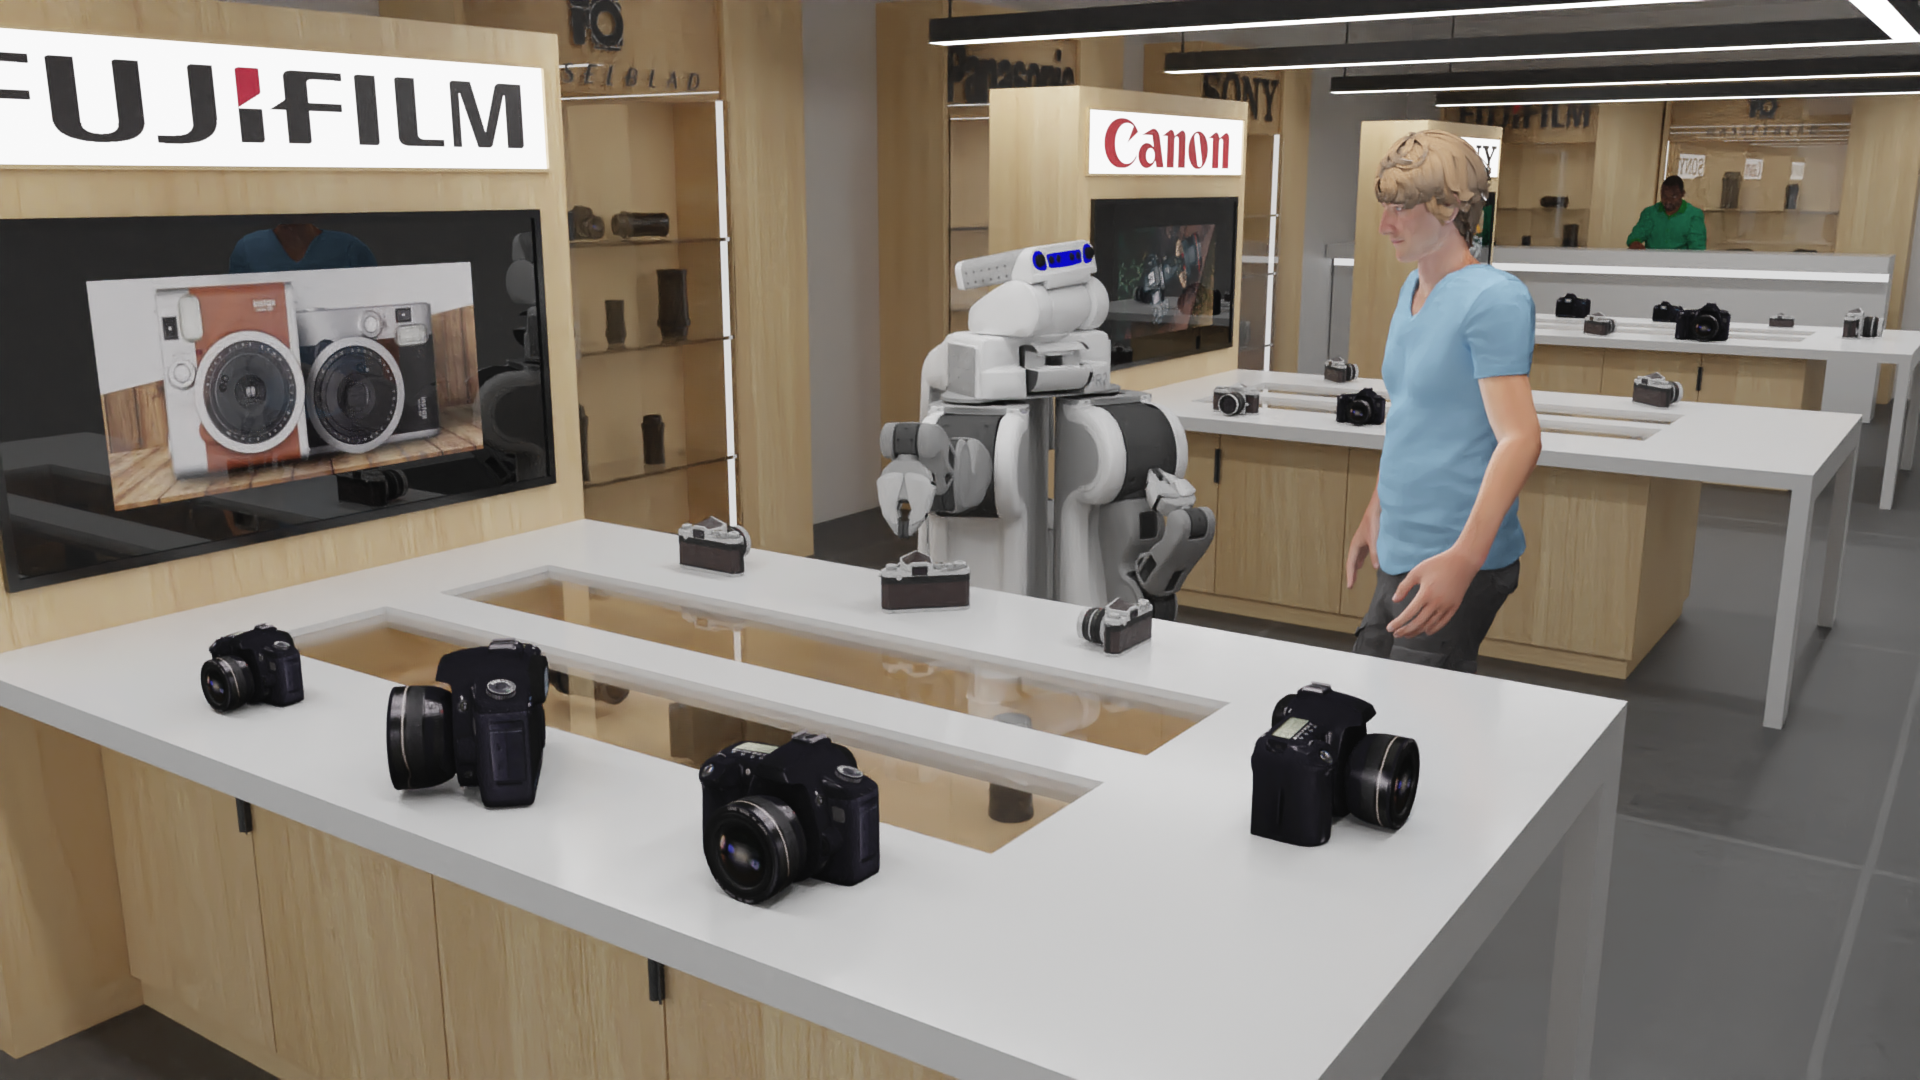
\includegraphics[width=\textwidth]{figures/introduction/camera_store_2.png}
\caption{\label{fig:cam_store} A Pr2 robot, as an employee of a camera store, advises a customer. }
\end{figure}

Explaining that, Max points to the cameras. They continue to discuss when Tony's phone rings. He has to go to join his wife, in another store in the mall. Not knowing where the other store is located, he asks:

\begin{quote}
\textit{
Tony - ``I am sorry I have to go. I will come back in the week. I have to go to a store selling video games but I do not remember the name.'' \\
Max - ``There is only one store selling video games in this mall, it is Game-ania.'' \\
Tony - ``Do you know how to reach it from there ?'' \\
Max - ``For sure''}
\end{quote}

Max moves next to the entrance, followed by Tony. It raises one arm pointing to the aisle and said:

\begin{quote} 
\centering 
\textit{
Max - ``Go down this aisle then turn left straight after the salad bar. After that Game-ania will be on your right when we walk.''}
\end{quote}

Tony leaves and comes back the morning after. Max recognizes him and moves towards him. It asks Tony if he has easily found the video game shop then recalls the camera identified the day before.

\begin{quote} 
\centering 
\textit{
Max - ``Yesterday we stop on two Fujifilm cameras and a Canon for your trip.''}
\end{quote}

They continue to discuss and finally Tony selects the camera at 350 euros. Following Max's advice, he takes a memory card and a second battery to have enough storage and power during his trip. In addition, he takes a zoom lens to take pictures of animals at long range. Unfortunately, the desired camera is not available at the moment. The last one in the store is the demonstration one. Max proposes to Tony to order the camera. The client agrees and leaves.

\begin{figure}[ht!]
\centering
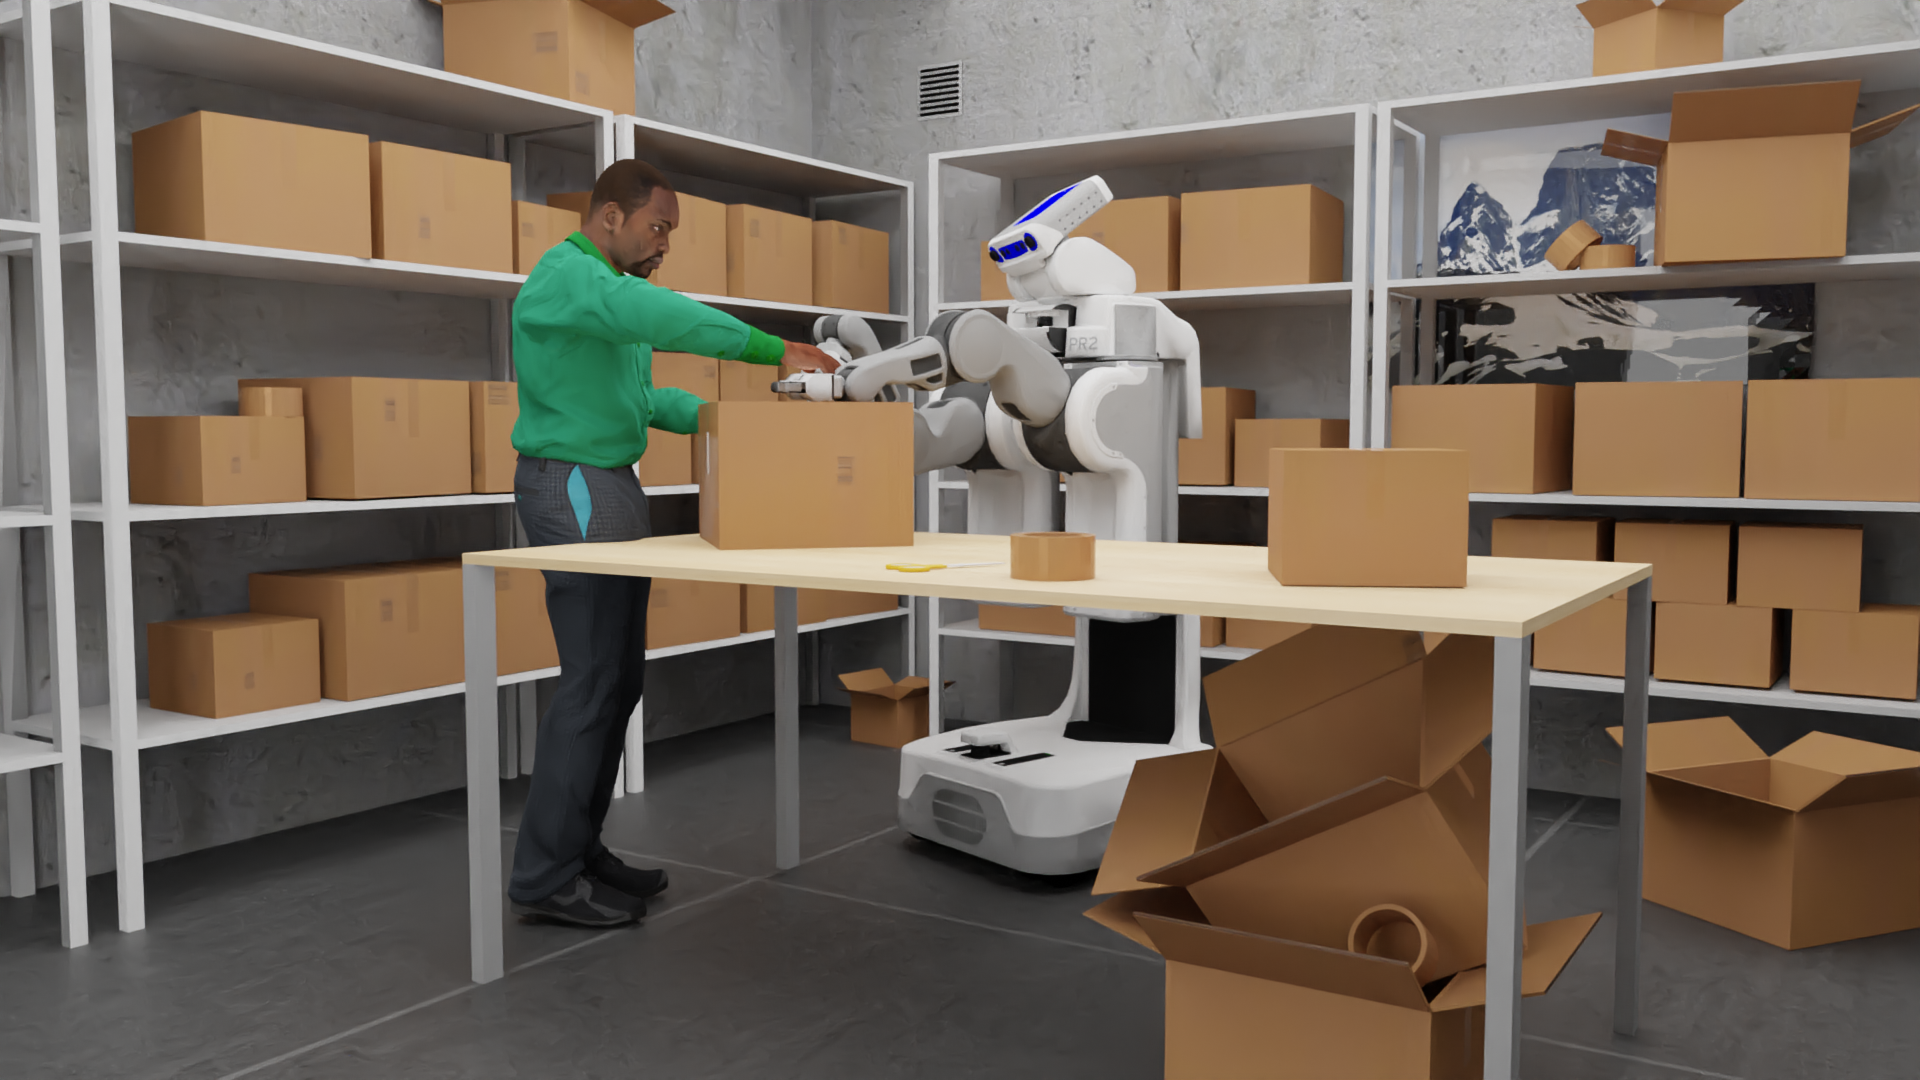
\includegraphics[width=\textwidth]{figures/introduction/camera_store_5.png}
\caption{\label{fig:cam_back} A Pr2 robot and a human employee collaborating to close a box. }
\end{figure}

A few days later, before opening, several boxes are delivered to the store. Liam, the human employee, and Max have to open them, fill stocks and prepare Tony's order. This is the first time since Max arrival they have to do it. They both go to the backroom in order to do this task together. There are two boxes. Liam starts opening one and so Max starts opening the other. Max informs Liam about the camera which has been ordered and is planned to be in the delivery.

\begin{quote} 
\centering 
\textit{
Max - ``Tell me if there is a X-T100, a customer orders one.''}
\end{quote}

Liam finds the camera. The robot explains to him that it also needs an SD card of 32Go and a lens XC 15-45mm. It informs the human that the SD cards are too small for it to grasp them. It thus proposes to Liam to take some of the cameras to put on the shelves and to bring back the card and the lens at the same time. During this time, Max gets a box, puts the camera and the battery inside. When Liam comes back, he puts the two other items in the same box. Then, Max maintains the box close while Liam tapes it. When finished, they both take the last items to put on the shelves and go to the main room.

The afternoon of the same day, while Max is cashing in a customer, Tony enters the store. Seeing him, Max requests Liam:

\begin{quote} 
\centering 
\textit{
Max - ``Can you bring the order we prepared this morning? The client is the one just entering, with the blue T-shirt.''}
\end{quote}

Liam goes to the backroom and brings back the correct box. Max charges the customer who finally gets his camera on time.

\section{Interacting with a robot: What can we expect ?}

Even if the scenario of the robot in a store is not intended to be entirely implemented, it allows us to identify what is needed in terms of knowledge representation, for a robot interacting with humans. First of all, we can draw a rough partition of the needed knowledge:

\begin{enumerate}
  \item \textbf{common-sense knowledge}. It is the knowledge not necessarily related to the current situation but required to understand it. In the scenario, this is not because the robot is in a camera store that it knows the concept of a camera, this concept is more general. Thanks to this common ground it is able to understand the concept of video games, trips, boxes, or animals in our scenario.
  \item \textbf{knowledge of the environment}, grounded in the space. The robot does not only need to know how it can move in its environment, it has to identify the elements composing it, link them to the common ground, and refine them. When Max is powered on for the first time, it goes around the environment to analyse it. Seeing an object, Max identifies it as being a camera. With additional cues, it can refine its knowledge through the model of this camera and its characteristics. This object is on a support, this is a shelf, dedicated to a specific brand, and so on.
  \item \textbf{knowledge of the activities}, grounded in the space and the time. More than how to perform a given task, we are here interested in how it has been achieved. By whom? With whom? Where? When? On which entities? In our scenario, Liam has brought back an SD card from the main room, during this time, Max has prepared a box in the backroom, and these two tasks have been made to prepare, together, Tony's command.
\end{enumerate}

Through this rough partition, we can identify three types of knowledge. The general ones, the knowledge related to space, and those related to time. Where the first can be seen as partially static, all have to be dynamic. The robot should be \textbf{able to gather knowledge}, update it, and create links in between.

At this stage, one can asks: where is the interaction in it? Even if this knowledge is mandatory for a robot interacting with a human, it holds also for a robot acting alone in an environment.

Speaking about interaction, the first use of the knowledge we can think about is communication, meaning sharing information. Consequently, an important property of the robot's knowledge is that a part of it has to be \textbf{narrative-enabled}. The robot should be able to communicate its knowledge. As humans, we can naturally think about verbal communication, for example when it explains the characteristics of the cameras. It can however also be through gestures, like pointing or other dietic gestures. When the robot says ``turn right'' while explaining a route to follow, the language can be accompanied by a hand gesture, turning it on the right. Moreover, for a robot equipped with a screen, we could also imagine communication through texts or images. We claim that only a part of its knowledge has to be narrative-enabled since another part can be dedicated to its internal functioning, from a pure engineering point of view.

When we qualify a piece of knowledge to be narrative-enabled, we can restrict ourselves to communication from the robot and to the human. However, if we consider the robot able to express knowledge, we can assume it to be able to understand it. In this way, in our conception of narrative-enabled knowledge, the robot should be able to formulate sentences and understand humans speech, based on its knowledge. Moreover, to understand its partner the robot not simply has to match the expressed concepts to its knowledge. Since some communications are underspecified, like when the client requests a camera for a trip, the robot can make use of \textbf{inference} to better understand the human. In our scenario, the client explains he is not an expert so the robot advises for an automatic camera. Since he goes on a trip, more storage and battery could be necessary. Since he wants to take pictures of animals, a zoom lens could be useful. All these pieces of information are not explicit to the communication, but thanks to inference on the knowledge can be understood by the robot. Finally, to fully understand its partner, the robot has to consider the \textbf{context} of the entire interaction. When Tony said he wants to acquire a camera at 350 euros, it seems trivial that it is the one at this price among the three previously identified.

Moving toward the knowledge about activities, we have to speak about \textbf{plans}. Keeping it simple for the moment, we can consider a plan as a succession of actions allowing an agent to achieve a task. In this way, a cooking recipe is a kind of plan allowing to achieve the task to prepare a dish. Through the narrative-enabled characteristic of knowledge, we thus want a robot to be able to express a plan. In our scenario, Max asked Liam to bring back an SD card and a lens, it thus expresses a part of a plan. However, it could also have explained to Liam to go in the main room, to move toward the second shelf, to open the rightmost door, to take the SD card in a blue package, and to come back in the backroom. This explanation expresses the same thing but goes deeper into the details, taking a lower level of \textbf{abstraction}. Here we see that the robot has to be able to express a plan at various levels of abstraction. For example, if the robot says ``Let us prepare the order'' it expresses the global task.

Such an explanation of a plan to be carried out highlights a number of key elements regarding the robot's need for knowledge. Here we introduce two of them:

\begin{itemize}
  \item If the robot can express the same plan with different granularity, how does it choose the right one? To answer this question, we have to introduce the self-and-other distinction. To know which information to share, a robot has to \textbf{estimate its partner knowledge}, that it is the common-sense knowledge as well as the knowledge about the environment and the activities. It is on the basis of this estimation that the robot can know how to communicate. In our scenario, the robot interacts with the human employee to prepare the order. Since Liam was in the store before the robot, it could estimate that the employee knows where the SD cards are. Communicating this low-level information would thus be useless and inefficient for the task. The human employee would be a new one, the robot would have interacted in a different way. This estimation of the others knowledge can be found somewhere else in the scenario. When Max refers to a specific camera to the client, it describes it in relation to its attributes and location. To the difference, to refer to the same entities to Liam, Max uses the precise model name of the camera. It thus estimates that the client does not know the model's name but that the employee does.
  
  \item To allow the robot to communicate at the right level of abstraction, estimating the other knowledge allows the detection of \textbf{belief divergence}. It appears when the robot estimates that the other does not have a piece of knowledge or still considers a piece of knowledge that no more holds. Detecting such a divergence can be used to prevent errors for example. In our scenario, if the robot has taken the last zoom lens on a given shelf and estimates that the employee is not aware of this information, it can detect a belief divergence. Consequently, rather than just asking for a zoom lens, it can inform the other that there is no more lens at this place. The employee will no have to search at the original place and will be able to directly go to another place where there is still some zoom lens.
\end{itemize}

Continuing to explore the knowledge implies by the realisation of a plan, we can move toward the elaboration of the plan, the planning of the task. By achieving the task together, the human and the robot are performing a \textbf{joint-task}, meaning having a joint-goal and collaborating to achieve it. To collaborate the robot elaborates a \textbf{plan considering the human}. It can thus propose to him to achieve a part of the task. To know how to dispatch the actions, the robot needs knowledge about \textbf{human abilities} as well as its own abilities. In the scenario, the SD card is assigned to the human because the robot is aware that it can not grasp it. If the object to bring back was graspable by it, maybe it would have done it by considering it as uncomfortable for the human to walk too much. Underlying, this ability to plan for himself and others also requires a projection into future situations and thus a \textbf{representation of possible worlds state}, like what is done in task planning.

Finally, the human is not an agent like the robot, he can not be controlled. Even if the robot plans by considering him, the human can act freely. The robot thus has to \textbf{monitor, interpret, and ground human actions}. From there and with regard to the plan and thus the joint-task, it can react and adapt. In our scenario, when Liam starts opening one of the two boxes, the robot adapts and takes the other one, even if it planned a different course of action. In this situation inverting does not raise any issue, they can thus continue.

In this section, we have identified some of the key elements need and use about knowledge for \acrfull{hri}. Even if we were not able to tackle all of them in this thesis, they give the context in which the presented contributions have been thought and they aim to be integrated. In this section, we have often use the term ``knowledge''. However under this general term can be found a number of concepts related to memory and how, as humans, we are able to remember things. Before moving to the contributions of this thesis, we propose in the next section an overview of some model from the cognitive psychology, allowing to better understand how we represent our knowledge.

\section[Knowledge organization]{Knowledge organization: Drawing inspiration from cognitive psychology }

Even if our goal in robotics is not to create a copy of the human, either in terms of body shape or cognition, drawing inspiration from it is nevertheless important. In the same way that roboticists take inspiration from the human body to create robots able to act in a world created by and for the human, the field of cognitive robotics takes inspiration from the human cognition to create robots able to interact with humans. While we do not aim to imitate human cognition, we think that a robot must be endowed with some similar capabilities if we want them to interact with us efficiently and in an acceptable way.

Regarding the knowledge representation, the first experimental study has been realized in 1885 by Ebbinghaus~\cite{ebbinghaus_1885_gedachtnis}. Since then, the definition of memory as the capacity to encode, store, and retrieve knowledge \cite{roediger_1996_retrieval} has been widely accepted. At the same time, the word ``memory'' has become a generic term suggesting a unique system. However, the human memory can rather be seen as several sub-systems that differ from their storage duration, storage capacity, and the level of consciousness necessary for information retrieval. In the rest of the section, we present some memory models, presented in a non-chronological way, and focussing on what is called long-term memory. During all this section, it is important to keep in mind that we only present models aiming to understand human cognition with a focus on knowledge management. No formal truth is stated here given that there is no consensus in the field. The presented models and terms will allow us to better understand the existing robotic cognitive architectures and give inspiration for the design and structuring of the components developed in this thesis.

The primary division of the memory is done concerning the storage duration and capacity. From there has been defined the \textbf{short-term memory} (STM) and the \textbf{long-term memory} (LTM) \cite{atkinson_1966_some}. Short-term memory is characterized by its small capacity and its capability to retrieve information that has just been seen. It is often stated that it is near to twenty seconds and seven items (or chunks)\cite{miller_1956_human}. Long-term memory, on the opposite, refers to any situation where we use information that has not just been seen. It is often stated that it has an infinite capacity and duration. It is this latter that allows the acquisition of new knowledge and the retrieval of information acquired a long time ago.

Over the years, what was called short-term memory has become the \textbf{working memory} (WM) \cite{baddeley_1986_dementia}. This change has been made to add a notion of knowledge manipulation. Instead of focusing on the only temporal aspect, it reflects its functional aspect. It is thus a system that retains information for the time necessary for its use by other cognitive functions. The working memory and the long-term memories are two independent but related systems. For information to be stored in long-term memory, we think that it has to pass by the working memory.

For the structure of the long-term memory, a first dichotomy is proposed by Graf and Schacter \cite{graf_1985_implicit} with the \textbf{implicit} and \textbf{explicit} memory. It reflects the way knowledge can be retrieved. Knowledge from explicit memory can be retrieved consciously and voluntarily. On the opposite, knowledge from implicit memory is retrieved in situations in which our behaviors are influenced by an experience. This is the case when one pours water into a glass. We do not need to retrieve explicitly how to perform this task. It is our experience that influences how we do it.

Another dichotomy has been proposed by Squire and Cohen \cite{squire_1982_remote} with the \textbf{procedural} and \textbf{declarative} memory. Procedural memory is the system allowing us to retain knowledge about our cognitive, motor, or perceptual skills. It is the memory of the know-how. A specificity of this memory is that it is difficult to verbalize the knowledge it stores and we use them unconsciously. The declarative memory stores representations of facts, events, general knowledge, and memories of past events. This knowledge can be retrieved consciously and we can speak about them. Taking the example of the code of your credit card. Initially, this knowledge is stored in the declarative memory. When you need it, you can easily remember it and say it. The more you use it and it slowly becomes an automatism. It became hard to remember it consciously while you use it every day and if you need to say it you need to type it on a virtual keyboard to remember it. It has slowly moved into your procedural memory. We see that both dichotomies are almost equivalent. The declarative memory of Squire is related to the implicit memory of Graf, and the procedural one is related to the implicit memory.

Going deeper into the declarative memory, Tulving has proposed a dichotomy between \textbf{episodic} and \textbf{semantic} memory \cite{tulving_1995_organization}. The episodic memory retains knowledge related to past experienced events, which are specific to our individual experience, and localized both in space and time. The semantic memory is more general and retains knowledge that we accumulate all along with our life concerning our environment. It can be seen as an encyclopedic memory independent of the acquisition context. While the episodic memory is related to ``remembering'', the semantic one is related to ``knowing''. Taking as an example your visit to Toulouse \footnote{If you never visit it, you can take another city you have visited but you should plan to visit it anyway.}, this visit is encoded in the episodic memory while the knowledge that Toulouse is a city in France is encoded in the semantic one.

\begin{figure}[h!]
\centering
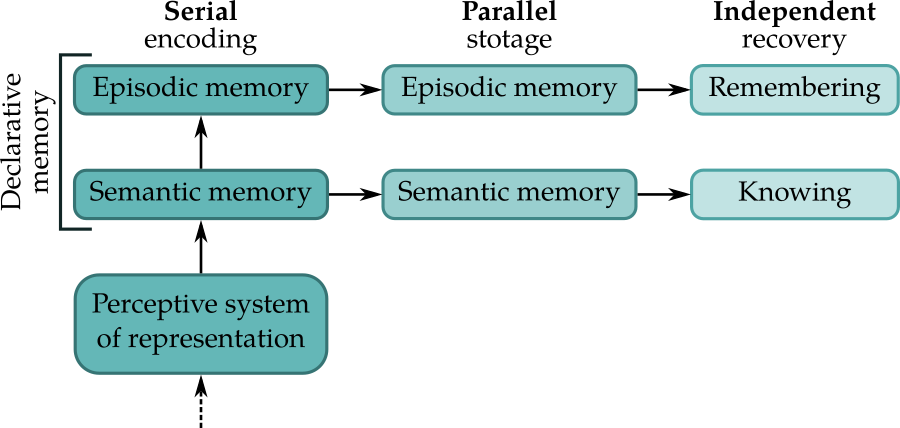
\includegraphics[scale=0.45]{figures/introduction/SPI.png}
\caption{\label{fig:SPI} Relations between episodic memory and semantic memory according to the SPI (Serial, Parallel, and Independent) model of Tulving (1995).}
\end{figure}

With the previous example, we saw that even if these two sub-systems of the declarative memory are independent, they are therefore in interaction with each other as we can apply a semantic treatment on the episodic memory. To better understand their relation, Tulving has proposed the Serial, Parallel, and Independent model (SPI). As illustrated in Figure~\ref{fig:SPI}, the encoding of information is serial (S) passing first by the semantic memory, then in the episodic one. The storage in both memories is performed in parallel (P). Finally, the information recovery is independent between the two memories.
As we explain at the beginning of this section, the presented theory can not be proven and must therefore be taken as~\cite{tulving_1995_organization} ``an explicit starting point for a more systematic pursuit of what is clearly the next problem that needs to be tackled''.

For this thesis, and robotic in general, these hypotheses about the knowledge organisation for humans allows a better understanding of the kind of knowledge we have to manage. We have identified three types: semantic, episodic, and procedural. Wanting to insert a new piece of knowledge, we can thus identify the types it is of and thus where to store it.

\section{Contributions}

This section summarizes the main contributions of this thesis. They are organised around three complementary topics: knowledge management, knowledge exploitation, and cognitive architectures. All have been thought in the context of \acrlong{hri}, meaning what a robot needs to take the human into account and interact with him.

\subsection{Knowledge management}

The starting point of this thesis is the need to store and maintain both the robot's and humans' estimated knowledge. We focused our efforts on semantic knowledge, using an ontology to represent it. The core contribution of this thesis is thus a software component to manage ontology instances. Each instance represents an agent knowledge, with the robot one being its ``ground truth''\footnote{This is the knowledge about what has been directly perceived by the robot.} and its partners' ones being an estimation of their knowledge\footnote{Either estimated to be perceived by the human or explicitly provided by the programmer.}. The ontology is used to represent the common-sense knowledge, the knowledge about the environment, knowledge about activities, as well as knowledge for the proper functioning of the robot.

The resulting software is called Ontologenius. It is a lightweight and open-source software developed in C++ and working as a server within a robotic architecture. Any component of the architecture can thus access the knowledge it maintains through the ROS middleware, ensuring uniformity of the knowledge among the entire architecture. It comes with extensive documentation, debugging tools, and an API in C++ and python.

Ontologenius supports dynamic updates of the \acrlong{kb}s it maintains and keeps them consistent at any instant thanks to reasoners. At the date, five main reasoners are available in the form of plugins, each dedicated to a specific axiom. Others can thus be added depending on the need. They can be activated or deactivated at runtime and propose different reasoning managements. We can for example choose to run then upon the query, at an update or periodically. Ontologenius is able to make the difference between a stated fact and a deduced one.

At the difference of other ontology management software, Ontologenius comes with more than 60 low-level inbuilt parametrizable queries, allowing a fast and precise exploration of the knowledge. These queries have been designed in such a way to be called from search algorithms to create higher-level cognitive processes. In addition, it proposes a \sparql{} interface.

Ontologenius has also been designed to be used for task planning applications by representing several possible world states in a single instance, switching from one to another.

It was made from scratch and thought like a sandbox, based on ontology standards but sometimes allowing to deviate from them to better explore the possibilities and never be limited.

During this thesis, a software to manage episodic knowledge has also been developed and linked with Ontologenius. It is called Mementar. Due to its early stage, it will not be presented in-depth but used in the final contribution of this thesis. 

\subsection{Knowledge exploitation}

On the basis of the semantic knowledge management software Ontologenius, several knowledge exploitation contributions have been developed. We can group them all into the topic of spatial referring.

The first tackles the route description task. Describing an indoor environment using an ontology, we have proposed two complementary algorithms able to find several routes leading to a target place. To represent an indoor environment with an ontology, we have proposed a piece of ontology to describe the topology, called the \acrlong{ssr}. It allows the description of the static elements of the environment, perceptible by humans, as well as elements necessary for the verbal description of a route. We have then developed an algorithm to verbalise routes, respecting good practices.

The second tackles the \acrlong{reg} task. The goal is to search for the knowledge to communicate to a hearer allowing him to identify the target entity without ambiguity, in a given context. The resulting algorithm has been shown as being the most efficient to date, even if the input \acrshort{kb} is not dedicated to the task. This contribution has been an important source of inspiration and has lead to three other related contributions. We have linked this algorithm to a symbolic task planner to evaluate communication feasibility and cost during the planning process. After this link with a planner, we tried to exploit the shared Human-Robot experience as a new kind of knowledge usable to generate \acrlong{re}. The latter contribution leads us to a proposal of task representation in an ontology. To move toward a more generic method to generate \acrlong{re}, we finally start a preliminary work aiming to support n-ary relations.

\subsection{Cognitive architectures}

The last contributions of this thesis are two cognitive architectures embodied on a Pepper and a Pr2 robotic platforms. The first architecture has been developed in the context of the \acrlong{mummer} project. It makes use of the route description to guide customers in a mall. The second has been developed later at LAAS-RIS to experiment recent developments of the team. This architecture makes use of the contributions around the \acrlong{reg}. It has been tested in a task inspired by cognitive psychology and adapted to the \acrlong{hri}, called the Director Task.

Both architectures use Ontolognenius to manage the robot and humans semantic \acrshort{kb}s. Since both architectures were developed two years apart, we will see in this thesis how the semantic \acrlong{kb} has become a central element of our cognitive architecture for \acrlong{hri}.

\section{A reader's guide}

\subsection*{Thesis organisation}

This thesis is partly based on published or submitted work. Some of the key contributions are more detailed than the paper version, while work involving several students is rather summarized to provide an overview of an integrated contribution.
This thesis is organised in an almost progressive way. Such an organisation aims at following step by step the way in which each contribution has been thought about regarding the previous ones. For example, from Chapter \ref{chap:5} to Chapter \ref{chap:7} an architecture is built proposing each time the integration of new components and new abilities. 

This thesis is organized into three parts: knowledge management, knowledge exploitation through referring applications, and finally the integration into robotic architectures. The knowledge management is presented in Chapter~\ref{chap:ontologenius} with the software Ontologenius. This software is then the core of all the other contributions. The knowledge exploitation has been studied with referring tasks. Chapter \ref{chap:3} proposes a knowledge representation and algorithm to describe routes for guide robots. Chapters \ref{chap:4} to \ref{chap:7} are all around the \acrlong{reg} problem. This thesis ends with two robotic architectures embodied respectively into a Pepper and a Pr2 robotic platform. The first architecture has been developed approximatively from 2017 to 2019 in the context of a European project. The second architecture is an internal project of the team, giving more flexibility to explore new designs and new organisation of its components. The latter has been developed from 2020 to 2021. While the first architecture uses the route description knowledge exploitation, the second use the contributions on the \acrlong{reg}. Having these two architectures grouped at the end of this thesis allows us to compare them and see how knowledge management has taken a primary place in a robotic architecture for \acrlong{hri} applications.

All along this thesis, special attention has been paid to the performance of each contribution. Each time our aim is to integrate the presented contribution into a wider system and work in an incremental manner. To not spoil the final Human-Robot interaction and be able to create more high-level cognitive capabilities, this attention is essential to us. At the end of most of the chapter, a performance analysis is thus provided.

\subsection*{To get to the point}

For the readers having less time and wanting to go to the point of this thesis, we can propose a shorter reading route. For sure, this selection is subjective, we often prefer our latter work, which seems to us more mature, having a better background on the topics. We thus suggest to read to following:

\begin{itemize}
  \item Chapter \ref{chap:ontologenius}: Ontologenius, the ontology management software, the core of this thesis,
  \item Chapter \ref{chap:4}: The \acrlong{reg} algorithm,
  \item Introductions of chapters \ref{chap:5} and \ref{chap:6}: Some challenges around the \acrlong{reg},
  \item Chapter \ref{chap:7}: A preliminary work to create more generic \acrlong{re}s,
  \item Section \ref{sec:9_3}: Our most advanced cognitive architecture for \acrlong{hri} applications.
\end{itemize}

\subsection*{List of Publications}
\markright{LIST OF PUBLICATIONS}
\subsubsection*{Published}
\begin{itemize}
\item Sarthou, G., Alami, R., \& Clodic, A. (2019, June). Semantic Spatial Representation: a unique representation of an environment based on an ontology for robotic applications. In Combined Workshop on Spatial Language Understanding (SpLU) and Grounded Communication for Robotics (RoboNLP).

\item Sarthou, G., Clodic, A., \& Alami, R. (2019, October). Ontologenius: A long-term semantic memory for robotic agents. In 2019 28th IEEE International Conference on Robot and Human Interactive Communication (RO-MAN) (pp. 1-8). IEEE.

\item Heikkilä, P., Lammi, H., Niemelä, M., Belhassein, K., Sarthou, G., Tammela, A., Clodic, A.,  \& Alami, R. (2019, November). Should a robot guide like a human? A qualitative four-phase study of a shopping mall robot. In International Conference on Social Robotics (pp. 548-557). Springer, Cham.

\item Buisan, G.*, Sarthou, G.*, Bit-Monnot, A., Clodic, A., \& Alami, R. (2020, August). Efficient, situated and ontology based referring expression generation for human-robot collaboration. In \textit{2020 29th IEEE International Conference on Robot and Human Interactive Communication (RO-MAN)} (pp. 349-356). IEEE.

\item Buisan, G., Sarthou, G., \& Alami, R. (2020, November). Human aware task planning using verbal communication feasibility and costs. In \textit{International Conference on Social Robotics} (pp. 554-565). Springer, Cham.
\end{itemize}

\subsubsection*{Accepted}

\begin{itemize}
\item Sarthou, G., Mayima, A., Buisan, G., Belhassein, K., \& Clodic, A. The Director Task: a Psychology-Inspired Task to Assess Cognitive and Interactive Robot Architectures. To be published in \textit{2021 30th IEEE International Conference on Robot and Human Interactive Communication (RO-MAN)}.

\item Sarthou, G., Buisan, G., A., Clodic, A., \& Alami, R. Extending Referring Expression Generation through shared knowledge about past Human-Robot collaborative activity. In \textit{2021 IEEE/RSJ International Conference on Intelligent Robots and Systems (IROS)}
\end{itemize}

\subsubsection*{Submitted}

\begin{itemize}
\item Mayima, A., Sarthou, G., Buisan, G., Singamaneni, P., Sallami, Y., Belhassein, K., Waldhart, J., Clodic, A., \& Alami, R. Direction-giving considered as a Human-Robot Joint Action. Submitted to \textit{User Modeling and User-Adapted Interaction (UMUAI) Journal}.
\end{itemize}
\ifdefined\included
\else
\setcounter{chapter}{1} %% Numéro du chapitre précédent ;)
\dominitoc
\faketableofcontents
\fi

\chapter{State od the art}
\minitoc

Lorem ipsum dolor sit amet, consectetur adipiscing elit. Sed non risus. Suspendisse lectus tortor, dignissim sit amet, adipiscing nec, ultricies sed, dolor. Cras elementum ultrices diam. Maecenas ligula massa, varius a, semper congue, euismod non, mi. Proin porttitor, orci nec nonummy molestie, enim est eleifend mi, non fermentum diam nisl sit amet erat. Duis semper. Duis arcu massa, scelerisque vitae, consequat in, pretium a, enim. Pellentesque congue. Ut in risus volutpat libero pharetra tempor. Cras vestibulum bibendum augue. Praesent egestas leo in pede. Praesent blandit odio eu enim. Pellentesque sed dui ut augue blandit sodales. Vestibulum ante ipsum primis in faucibus orci luctus et ultrices posuere cubilia Curae; Aliquam nibh. Mauris ac mauris sed pede pellentesque fermentum. Maecenas adipiscing ante non diam sodales hendrerit.

\section{Congnitive architectures and underlying knowledge representations}

\section{How reasoning can expand the knowledge}

\section{Knowlege exploitation for service robotics}

\section{Knowlege exploitation for Human-Robot Interaction}

Lorem ipsum dolor sit amet, consectetur adipiscing elit. Sed non risus. Suspendisse lectus tortor, dignissim sit amet, adipiscing nec, ultricies sed, dolor. Cras elementum ultrices diam. Maecenas ligula massa, varius a, semper congue, euismod non, mi. Proin porttitor, orci nec nonummy molestie, enim est eleifend mi, non fermentum diam nisl sit amet erat. Duis semper. Duis arcu massa, scelerisque vitae, consequat in, pretium a, enim. Pellentesque congue. Ut in risus volutpat libero pharetra tempor. Cras vestibulum bibendum augue. Praesent egestas leo in pede. Praesent blandit odio eu enim. Pellentesque sed dui ut augue blandit sodales. Vestibulum ante ipsum primis in faucibus orci luctus et ultrices posuere cubilia Curae; Aliquam nibh. Mauris ac mauris sed pede pellentesque fermentum. Maecenas adipiscing ante non diam sodales hendrerit.

Ut velit mauris, egestas sed, gravida nec, ornare ut, mi. Aenean ut orci vel massa suscipit pulvinar. Nulla sollicitudin. Fusce varius, ligula non tempus aliquam, nunc turpis ullamcorper nibh, in tempus sapien eros vitae ligula. Pellentesque rhoncus nunc et augue. Integer id felis. Curabitur aliquet pellentesque diam. Integer quis metus vitae elit lobortis egestas. Lorem ipsum dolor sit amet, consectetuer adipiscing elit. Morbi vel erat non mauris convallis vehicula. Nulla et sapien. Integer tortor tellus, aliquam faucibus, convallis id, congue eu, quam. Mauris ullamcorper felis vitae erat. Proin feugiat, augue non elementum posuere, metus purus iaculis lectus, et tristique ligula justo vitae magna.
Aliquam convallis sollicitudin purus. Praesent aliquam, enim at fermentum mollis, ligula massa adipiscing nisl, ac euismod nibh nisl eu lectus. Fusce vulputate sem at sapien. Vivamus leo. Aliquam euismod libero eu enim. Nulla nec felis sed leo placerat imperdiet. Aenean suscipit nulla in justo. Suspendisse cursus rutrum augue. Nulla tincidunt tincidunt mi. Curabitur iaculis, lorem vel rhoncus faucibus, felis magna fermentum augue, et ultricies lacus lorem varius purus. Curabitur eu amet.

\ifdefined\included
\else
\setcounter{chapter}{2} %% Numéro du chapitre précédent ;)
\dominitoc
\faketableofcontents
\fi

\chapter{Ontologenius: A long-term semantic memory}
\minitoc

\section{Design and features}

\subsection{Why an ontology?}

\subsection{Ontology formalism}

Even if we saw that the use of ontology is today a common way to represent semantic knowledge, we will recall in this subsection the composition of an ontology. For each element composing it, we will draw a formalization then give examples using the Turtle syntax. The pieces of ontologies used in the examples of this subsection are voluntarily simplified. The introduced notations will be the ones used in the rest of this thesis and the graphical representations, both in terms of color and form, will be kept as often as possible.

On the base of the definition of a Description Logic ontology presneted in \cite{fokoue_2006_summary}, we define a semantic knowledge base $\kbs$ represented as an ontology by  $\kbs = \langle \Abox, \Tbox, \Rbox \rangle$. $\Abox$, $\Tbox$, and $\Rbox$ are respectively called the Abox, Tbox, and Rbox of the ontology.


\begin{figure}[h!]
\centering
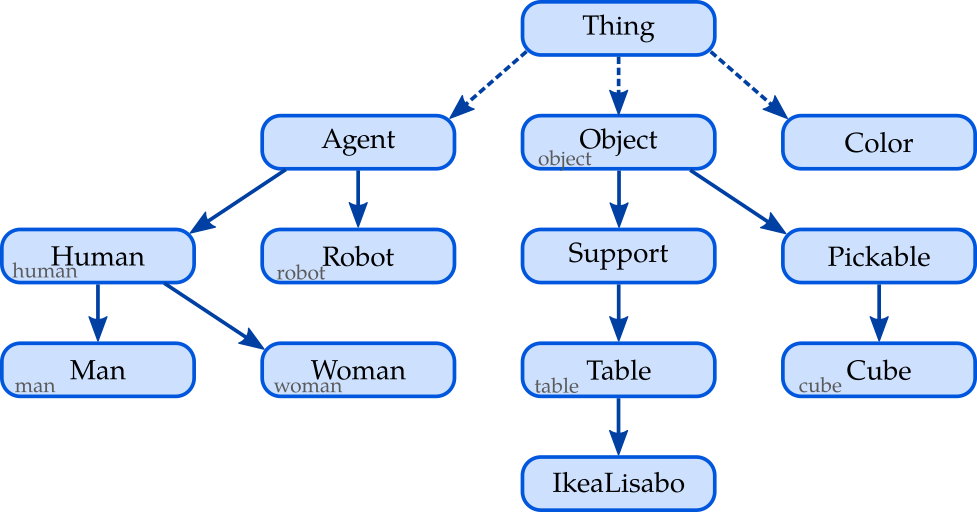
\includegraphics[scale=0.4]{figures/chapter2/Tbox.png}
\caption{\label{fig:Tbox} Representation of an ontology class hierarchy graph to illustrate the composition of a TBox. Taking the class Human, the bottom arrow has to be read as \textit{"A man is a kind of Human"}. The texts at the bottom left of the class, if there is, are the classes' labels in natural language.}
\end{figure}

The Tbox $\Tbox$ contains assertions about the \textbf{classes} (types) of the ontology. It is defined by $\Tbox = \langle \classset, H \rangle$. It can be seen as a directed acyclic graph as presented in Figure~\ref{fig:Tbox}. $\classset$ is the set of all the classes of the ontology. In our example, $\classset = \{Thing,\ Agent,\ Object, ...,\ IkeaLisabo\}$. Considering the Tbox as a graph, $H$ stores its directed edges. It represents the inheritance links between the classes (i.e. the subsumption assertions). This link is commonly referred to as the "isA" link (e.g. \textit{(Human, isA, Agent)}) and is described with the property rdfs:subClassOf in the OWL language as illustrated in the Listing~\ref{lst:Tbox}.

\begin{lstlisting}[frame=single, basicstyle=\scriptsize\ttfamily, label={lst:Tbox}, caption={Description of ontology classes in the OWL language using the Turle syntax.},captionpos=b]
:Human rdf:type owl:Class ;
       rdfs:subClassOf :Agent .

:Man   rdf:type owl:Class ;
       rdfs:subClassOf :Human .
\end{lstlisting}

\begin{figure}[h!]
\centering
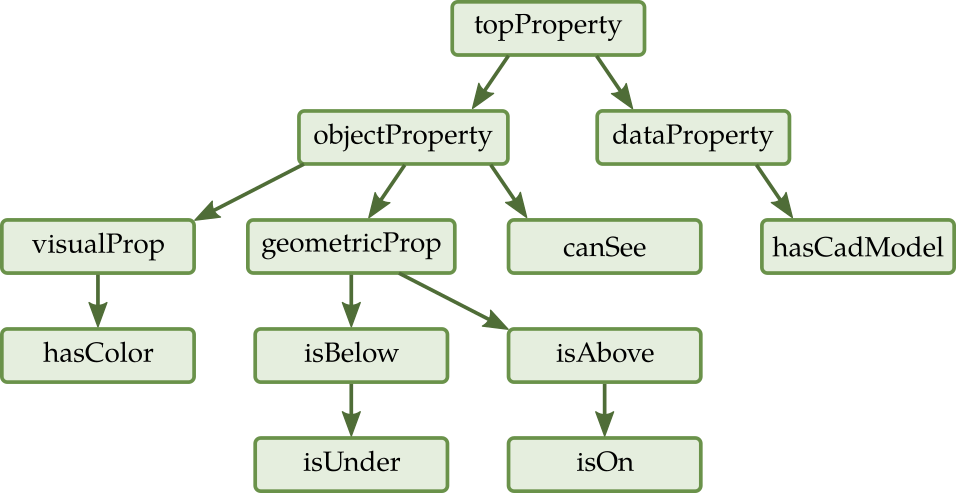
\includegraphics[scale=0.4]{figures/chapter2/Rbox.png}
\caption{\label{fig:Rbox} Representation of an ontology property hierarchy graph to illustrate the composition of an RBox. Taking the property isBelow, the bottom arrow has to be read as: \textit{"The property isUnder is a specification of the property isBelow"}.}
\end{figure}

The Rbox $\Rbox$ contains assertions about the \textbf{properties} (roles). It is at least defined by $\Rbox = \langle \propset, \inclset, \invset, \domainset, \rangeset \rangle$. In the same way as the Tbox, $\propset$ is the set of properties, and $\inclset$ stores the directed edges of the finite directed acyclic graph representing the inheritance links between the properties. Such a graph is represented in Figure~\ref{fig:Rbox}. These inheritance links aim at specifying properties. In our example, the property IsOn is a specification of the property isAbove in the way that an object being on another is an object that is above the latter and being in contact with. It is described with the property rdfs:subPropertyOf in the OWL language. 
$\invset = \{(\property, \property^{-1}) \in \propset^2\}$ is the set representing the properties inverses (\textit{e.g.} $(isOn, isUnder) \in Inv$). Describing the inverse of a property is useful first to reduce description work since if some describe a relation involving a property for which an inverse is defined, the inverse relation is also described in an underlying way. Moreover, for an algorithm exploring an ontology, knowing that a relation uses a property having an inverse can allow reducing the algorithm complexity by not considering the inverse relation into the exploration.
Finally, $\domainset$ and $\rangeset$ are two sets representing respectively the properties domains and ranges. Their are define by $\domainset = \{(\property, \class)\}$ and $\rangeset = \{(\property, \class)\}$ with $\property \in \propset$ a property and $\class \in \classset$ a class. The domain of a property informs on the type of resources that may use the property, thus the type of the subject of a triplet. The range of a property informs on the valid values applied to the property, thus the type of the object of a triplet. For the property isOn, we would therefore have $(isOn,\ Object) \in \domainset$ and $(isOn,\ Support) \in \rangeset$. In this way, we state that the property IsOn can be used to describe that an object is on top of an object being support. Domains and ranges can be used in two ways. It can be to check the consistency of an ontology by checking if the way the properties have been used corresponds to their definition. It can also be used to reason on the ontology and extract new knowledge from a given situation. If, for example, an entity is said to be on top of another that is not described as being a support, we could deduce that this second entity may be a support.

The formalization above considers only a general kind of property while the OWL language makes the distinction between two main categories. The \textbf{object properties}, linking two entities, and \textbf{data properties}, linking an entity to a value. While both are slightly different, we will only keep a general definition of a property for our formalization to simplify the future algorithm explanations. An example of the description of an object property and a data property from the Figure~\ref{fig:Rbox} are illustrated in the Listing~\ref{lst:Rbox} using the OWL language.


\begin{lstlisting}[frame=single, basicstyle=\scriptsize\ttfamily, label={lst:Rbox}, caption={Description of ontology properties in the OWL language using the Turle syntax.},captionpos=b]
:isOn  rdf:type owl:ObjectProperty ;
       rdfs:subPropertyOf :isAbove ;
       owl:inverseOf :isUnder ;
       rdfs:domain :Object ;
       rdfs:range :Support .

:hasCadModel rdf:type owl:DatatypeProperty ;
             rdfs:domain :Object .
\end{lstlisting}

\begin{figure}[h!]
\centering
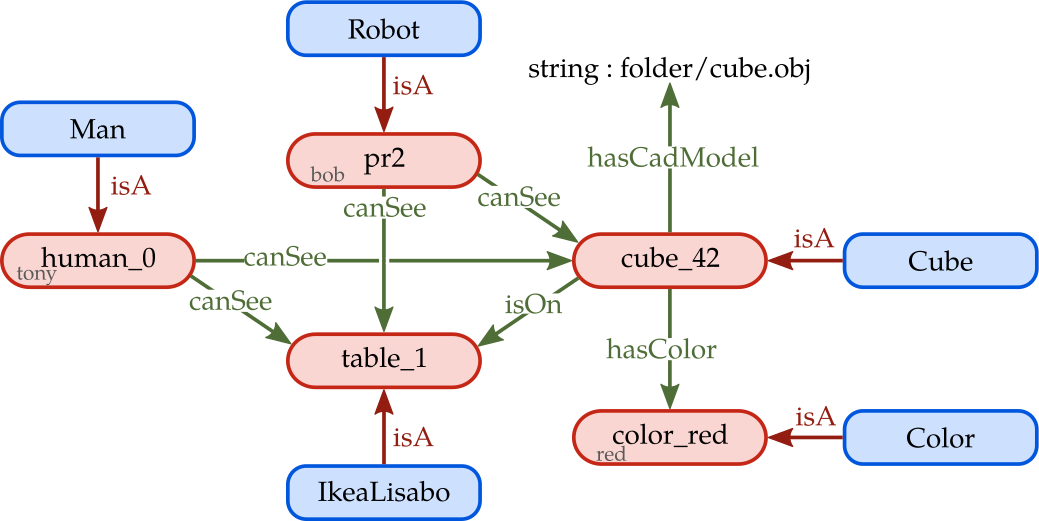
\includegraphics[scale=0.4]{figures/chapter2/Abox.png}
\caption{\label{fig:Abox}  Representation of an ontology instances graph to illustrate the composition of an ABox. Red boxes are individuals of the ontology. Green arrows are properties coming from the RBox and applied to individuals. Red arrows represent a direct inheritance link between an individual and a class coming from the TBox. The texts at the bottom left of the individuals, if there is, are the individuals' labels in natural language.}
\end{figure}

The Abox $\Abox$ contains assertions about the \textbf{entities} (individuals) of the ontology. When we refer about entities, we no more speak about general concepts but rather of instantiated concept, being either a physic or virtual entity. The Abox is defined by $\Abox = \langle \indivset, \inheritset_0, \relationset \rangle$. $\indivset$ is the set of all the entities represented in the ontology. $\inheritset_0$ the set of direct types of $\indivset$ such as $\inheritset_0 = \{(\indiv, \class) \}$ with $\indiv \in \indivset$ an individual and $\class \in \classset$ a class. In the graphical representation of an Abox in the Figure.~\ref{fig:Abox}, the red blocks are the Abox entities ($\indivset = \{human_0,\ pr2,\ ...,\ table\_1\}$) and the red arrows with the label "isA" are the intities direct types ($(cube\_42, Cube) \in \inheritset_0$).
$\relationset$ is finally the set of \textbf{relations} between entities. Such relation are in the form of triplets $(\subject, \property ,\object)$ where $\subject$ is the subject, $\property$ the property and $\object$ the object. The set of relations is thus defined by $\relationset = \{(\subject, \property ,\object) | (\subject, \object) \in \indivset^2, \property \in \propset\}$. These relations are represented by the green arrows between the entities in Figure~\ref{fig:Abox}. We can note in this figure the presence of the use of a data property "hasCadModel". This property does not link two entities, which goes against the previous definition. Regarding our formalization and to keep it tractable, we can however keep it as it is, and view the string value as an entity having for direct type a concept "String". An example of the description of an entity from the Figure~\ref{fig:Abox} is illustrated in the Listing~\ref{lst:Abox} using the OWL language.

\begin{lstlisting}[frame=single, basicstyle=\scriptsize\ttfamily, label={lst:Abox}, caption={Description of an ontology individual in the OWL language using the Turle syntax.},captionpos=b]
:cube_42  rdf:type     :Cube ;
          :hasColor    :color_red ;
          :hasCadModel "folder/cube.obj"^^string ;
          :isOn        :table_1 .
\end{lstlisting}


We just saw that in the Abox, $\inheritset_0$ contains the direct types of entities. We also saw that the classes can inherit from one each other in the Tbox, thanks to the classes inheritance directed edges stored in $H$. This means that the individuals of the Abox have inherited types. Taking the entity cube\_42 of Figure.~\ref{fig:Abox}, its direct type is the class Cube ($(cube\_42,\ Cube) \in \inheritset_0$). Regarding the Tbox represented in Figure.~\ref{fig:Tbox}, a Cube is a kind of Pickable ($(Cube,\ Pickable) \in H$), itself being a kind of Object ($(Pickable,\ Object) \in H$). We can thus say that the entity cube\_42 is a Cube, a Pickable, and an Object. To represent it, we use $\inheritset$ to denote the set of direct and inherited types. We thus have $\{ (cube\_42,\ Cube), (cube\_42,\ Pickable), (cube\_42,\ Object)\} \subset \inheritset$.

With the use of the relation set $\relationset$ of the Abox we saw that we can apply properties to individuals to link them together and form relations in the form of triplets. However, some could want to apply properties to classes to describe general links between classes. While properties domains and ranges already give such relations this can be not enough. Taking an object property hasMother, we can assign to it the class Human for domain and Woman for range. With such description, we state that a human CAN have a mother that is a woman but we do not describe that even if we do not know how it is, a human has a mother how is a woman. For this particular example, we could use cardinality constraint but we will not go as far. Taking now the data property hasCadModel of Figure~\ref{fig:Rbox}, we have applied it to a specific entity in the example of Figure~\ref{fig:Abox}. But what about a Table Lisabo (IkeaLisabo in Figure~\ref{fig:Tbox})? Any table of this model will have the same CAD model and we do not want to put this relation to every entity of this type of table. Here domains and range are not sufficient to represent it. To do so, we will use \textbf{annotation properties} applied to classes. Annotation properties are usually used to document ontologies and not to describe general relations on classes. We take thus some liberty regarding the OWL standard for convenience. However, we will try to use it in very particular cases where no other simple solution can be applied. Relations to classes using annotation properties are thus added to the definition of a Tbox $\Rbox = \langle \propset, \inclset, \invset, \domainset, \rangeset, \annotationset \rangle$, where $\annotationset$ is the set of relation between classes in the form of triplets.

In this sub-section, we have draw a formalism of an ontology in the form of $\kbs = \langle \Abox, \Tbox, \Rbox \rangle$. All the knowledge stored in $\kbs$ are sufficient to build exploration algorithm on top of it. However, to reason on ontology aditional descriptions are necessary in the form of properties characteristics. We do not add them to the knowledge base formalism but enumerate them bellow: 

\begin{itemize}
	\item \textbf{Symmetric property}: If the relation $(x, p, y)$ holds in $\relationset$ with $p$ being a symmetric property, the relation $(y, p, p)$ is also part of $\relationset$.
	\item \textbf{Asymmetric property}: If the relation $(x, p, y)$ holds in $\relationset$ with $p$ being an asymmetric property, the relation $(y, p, p)$ can no be part of $\relationset$.
	\item \textbf{Reflexive property}: A reflexive property can be used to link an individual to itself.
	\item \textbf{Irreflexive property}: An irreflexive property can not be used to link an individual to itself.
	\item \textbf{Functional property}: Every individual can be linked by a functional property to at most one other individual. By this way, if ${(x, p, y), (x, p, z)} \subset \relationset$, then $y = z$.
	\item \textbf{Inverse functional property}: Every individual can holds an iverse functional property at most one.  By this way, if ${(x, p, y), (z, p, y)} \subset \relationset$, then $x = z$.
	\item \textbf{Transitive property}: A transitive property describe a link between two individuals x and z whenever it exist a link between x and y, and y with z with this property. If ${(x, p, y), (y, p, z)} \subset \relationset$ with p a transitive property, then $(x, p, z) \in \relationset$.
	\item \textbf{Property chain axiom}: While the transitive property characteristic decsribe a link between several individuls with the same property, the chain axiom does the same with distinct properties. Given the chain $p_1 \bullet p_2 \Rightarrow p_3$, if ${(x, p_1, y), (y, p_2, z)} \subset \relationset$, then $(x, p_3, z) \in \relationset$.
	\item \textbf{Disjoinction}: Given two disjoint elements (classes or properties), a third element can not inherit of the both disjoint elements.
\end{itemize}

We saw in the previous chapter that the semantic knowledge base is part of what we assimilate to be the declarative memory. The particularity of such memory is the ability to speak about the knowledge it stores. In this way, we introduce a labeling function $\labelfunc$ for any element of the ontology. This labeling function is specified for the individuals ($\alabel$), the classes ($\tlabel$), and the properties ($\plabel$). Considering the individuals labeling function $\alabel: \indivset \rightarrow Lbl$ with $Lbl$ a set of communicable names encoded as UTF8 string in our implementation. The same holds for the other two labeling functions.

The ontology definition used all along this thesis is summarized in Table~\ref{tab:onto_symboles}.

\begin{table}[h]
\caption{The list of symbols of used to define a semantic knowledge base as an ontology }
\label{tab:onto_symboles}
\begin{tabular}{ll}
{\ul \textbf{$\Abox$ ABox entities/indiv}} & {\ul \textbf{$\Tbox$ TBox classes/concepts}}  \\
$\indivset$: set of entities               & $\classset$: set of classes  \\
$\inheritset_0$: entities' direct types        & $H$: classes inheritance links \\
$\relationset$: relations between entities    & $\annotationset$: relations between classes  \\
$\alabel$: individuals labeling function & $\tlabel$: classes labeling function \\
 & \\
\multicolumn{2}{l}{{\ul \textbf{$\Rbox$ RBox roles/properties}}}                          \\
$\propset$: set of properties              &                                              \\
$\inclset$: properties inheritance links       & $\invset$: properties inverses                   \\
$\domainset$: properties' domains sets     & $\rangeset$: properties' ranges sets   \\
$\plabel$: properties labeling function & \\
\end{tabular}
\end{table}


\subsection{Desired features}


\section{Architecture}

\subsection{Permanent versus temporary data structure}

\subsection{Concepts' identifier versus name in natural language}

\subsection{Resoning to enrich the knowledge}



\section{Managing others' estimated knowledge}

\subsection{Ontologenius multi-instances principle}

\subsection{Catching knowledge at a given moment}

\subsection{Exploring several possible mental states at once}



\section{Using Ontologenius in robotic applications}

\subsection{Inserting new knowledge}

\subsection{Retrieving knowledge}

\subsubsection{Low-level queries}

\subsubsection{SPARQL-like interface}

\subsection{The Application Programming Interface}

\subsubsection{Debbuging tool}



\section{Computational preformance evaluation}

\subsection{Concepts recovery}

\subsection{Low-level queries}

\subsection{SPAQRL queries}

Lorem ipsum dolor sit amet, consectetur adipiscing elit. Sed non risus. Suspendisse lectus tortor, dignissim sit amet, adipiscing nec, ultricies sed, dolor. Cras elementum ultrices diam. Maecenas ligula massa, varius a, semper congue, euismod non, mi. Proin porttitor, orci nec nonummy molestie, enim est eleifend mi, non fermentum diam nisl sit amet erat. Duis semper. Duis arcu massa, scelerisque vitae, consequat in, pretium a, enim. Pellentesque congue. Ut in risus volutpat libero pharetra tempor. Cras vestibulum bibendum augue. Praesent egestas leo in pede. Praesent blandit odio eu enim. Pellentesque sed dui ut augue blandit sodales. Vestibulum ante ipsum primis in faucibus orci luctus et ultrices posuere cubilia Curae; Aliquam nibh. Mauris ac mauris sed pede pellentesque fermentum. Maecenas adipiscing ante non diam sodales hendrerit.

Ut velit mauris, egestas sed, gravida nec, ornare ut, mi. Aenean ut orci vel massa suscipit pulvinar. Nulla sollicitudin. Fusce varius, ligula non tempus aliquam, nunc turpis ullamcorper nibh, in tempus sapien eros vitae ligula. Pellentesque rhoncus nunc et augue. Integer id felis. Curabitur aliquet pellentesque diam. Integer quis metus vitae elit lobortis egestas. Lorem ipsum dolor sit amet, consectetuer adipiscing elit. Morbi vel erat non mauris convallis vehicula. Nulla et sapien. Integer tortor tellus, aliquam faucibus, convallis id, congue eu, quam. Mauris ullamcorper felis vitae erat. Proin feugiat, augue non elementum posuere, metus purus iaculis lectus, et tristique ligula justo vitae magna.
Aliquam convallis sollicitudin purus. Praesent aliquam, enim at fermentum mollis, ligula massa adipiscing nisl, ac euismod nibh nisl eu lectus. Fusce vulputate sem at sapien. Vivamus leo. Aliquam euismod libero eu enim. Nulla nec felis sed leo placerat imperdiet. Aenean suscipit nulla in justo. Suspendisse cursus rutrum augue. Nulla tincidunt tincidunt mi. Curabitur iaculis, lorem vel rhoncus faucibus, felis magna fermentum augue, et ultricies lacus lorem varius purus. Curabitur eu amet.


\ifdefined\included
\else
\setcounter{chapter}{3} %% Numéro du chapitre précédent ;)
\dominitoc
\faketableofcontents
\fi

\chapter{Searching for a route with semantic knowledge}
\chaptermark{Searching for a route with an ontology}
\label{chap:3}
\minitoc

The contribution presented in this chapter is excerpted from our work, published in the proceedings of the Spatial Language Understanding (SpLU) 2019 workshop~\cite{sarthou_2019_semantic}. In this manuscript, the contribution is more detailed and discussed. This work is part of the MuMMER project, aiming at developing a robot guide in a mall. At the end of this thesis, a chapter is dedicated to the presentation of the project and the integration of the current contribution is a robotic system.

\section{Introduction}

We all have already been requested, or have ourselves request, for a route toward public space in a city, a shop in a shopping centre, or more simply a toilet in a house. When providing such information to a lost person we perform what is commonly called a guidance task. Even if it can seem evident for us, developing a robot able to perform it can be challenging. In this chapter, we choose to focus on the sub-task consisting to generate the explanation sentence. This sub-task is called the route description. To perform it, we first need a set of knowledge about the environment in which the guided person will walk, such as the paths, the intersections of the paths, or the elements alongside them. Then, we need a set of "good practices" to provide a route easy enough to follow and to remember.

In the Human-Robot Interaction (HRI) field, robots guides have been study intensively and deployed into shopping centers~\cite{okuno_2009_providing}, museums~\cite{burgard_1999_museum, clodic_2006_rackham, siegwart_2003_robox}, or airport~\cite{triebel_2016_spencer}. From a knowledge representation point of view, we can notice the use of metrical representations~\cite{thrun_2007_simultaneous} or topological representations~\cite{morales_2011_modeling} to represent the environment in which the robot evolves. Since we focus on the route description task, we consider that the robot does not accompany the human to his final destination but rather explains how to reach it. Consequently, the metrical representation will not be considered as being mainly used for navigation purpose~\cite{thrun_2007_simultaneous}. To perform more specifically a route description, topological knowledge is not sufficient. In addition to the topology of the environment, the robot needs to know the types of the elements composing the environment and their names in natural language. Some contributions have thus try to mix metrical or topological representations with semantic ones to hold this additional knowledge~\cite {satake_2015_should, chrastil_2014_cognitive, zender_2008_conceptual}. However, mixing them can create a lack of uniformity among the overall knowledge representation. In this way, creating a unique representation allowing a robot to compute routes and expressing them could ensure uniformity among the knowledge.

Even having a rich enough representation of its environment, the robot has to find a route not for it but for the guided human. A robot accompanying the human only has to determine a path, adapted to its capacities and interpretable only by it. Providing a route to a human, the route has to be adapted to the human capabilities. For example, in an outdoor environment, we will not give the same route for a car driver or a cyclist. In the context of a mall, we will not give a route with stairs along to a mobility-impaired person or to someone with a shopping cart. Once an adapted route computed, the robot has to explain it. Where interactive maps only have to highlight a path, here, the robot has to generate a sentence that the human will memorize. For sure the robot will not instruct a human with a sentence like "walk 30 meters them turn -90 degrees". This would not be adapted. The use of orientation and reference to elements of the environment will be needed through a sentence like "walk until the florist then turn left".

The first contribution of this chapter is a \textbf{unified representation} of an indoor environment using an ontology, to include both topological and semantic knowledge. Then, on the basis of this representation, we propose a first algorithm to \textbf{find a suitable route} to be explained to a human and a second algorithm to \textbf{verbalize a route} in an appropriate way.

First, we review the literature concerning semantic representation of indoor environment and route description. Then, we introduce the reader to our unified semantic representation under the name of Semantic Spatial Representation (SSR). We then present the algorithm used to compute the route and in a second time the algorithm to verbalize the previously computed route. We end this chapter with experimental results on both emulated and real environments.

\section{Related work}

\subsection{Describing a route}

In the literature, a route description task is defined as being a particular kind of spatial description. First, from a cognitivist point of view, Denis in~\cite{denis_1997_description} has identified three main cognitive operations used to generate such a spatial discourse: 1) the activation of an internal representation of the environment, 2) the planning of a route in this representation, 3) and finally the formulation of the procedure to follow. From a computer science point of view, Cassell in~\cite{cassell_2007_trading} view the second operation as the fact of finding a set of routes segment, each connecting two important points, and the third operation as chronologically explaining the route segments. In the same way, Mallot in~\cite{mallot_2009_embodied}, see the second operation as the fact of selecting a sequence of places leading to the objective, and the third as managing declarative knowledge to choose the right action to explain at each point of the sequence. While both second operations are equivalent, the thirds about the formulation of the procedure are rather complementary.

The route description task has been extensively studied through verbal and textual communication to understand how humans communicate spatial knowledge. The goal of such studies has been to identify the invariants but also the good practices ensuring the success of the task. Through five experiments in both urban and interior environments, Allen is~\cite{allen_2000_principles} has identified three basic practices seen as being important for communicating knowledge about routes. They can be summarized as follows: a) respect the spatiotemporal order, b) concentrate on the information about the points of choice and c) use landmarks that the listener can easily identify.

This latter practice about the use of landmarks, also called reference marks, has been identified by Tversky in~\cite{tversky_1999_pictorial} has been critical information for the success of a route description. With his anterior contribution~\cite{tversky_1998_space}, he finds that in addition to information about actions, reorientation, and direction, 91\% of the guidance instructions contains the use of landmarks. These results trend at confirming the ones of Denis in~\cite{denis_1997_description}. In an anterior study, Montello in~\cite{montello_1993_scale} tries to identify when the use of landmarks appear in a description. Defining the \textit{Vista} space as being the area within sight and the \textit{Environmental} as being the rest of the environment reachable through locomotion, he finds that guides usually used landmarks when the target places were no longer in the \textit{Vista} space but in the \textit{Environmental} one. Moreover, with regard to~\cite{tversky_1999_pictorial}, the use of landmark more precisely appears during an explanation of a direction changing. In addition, their choice is based on salient features over a route description~\cite{nothegger_2004_selection}.

\begin{figure}[ht!]
\centering
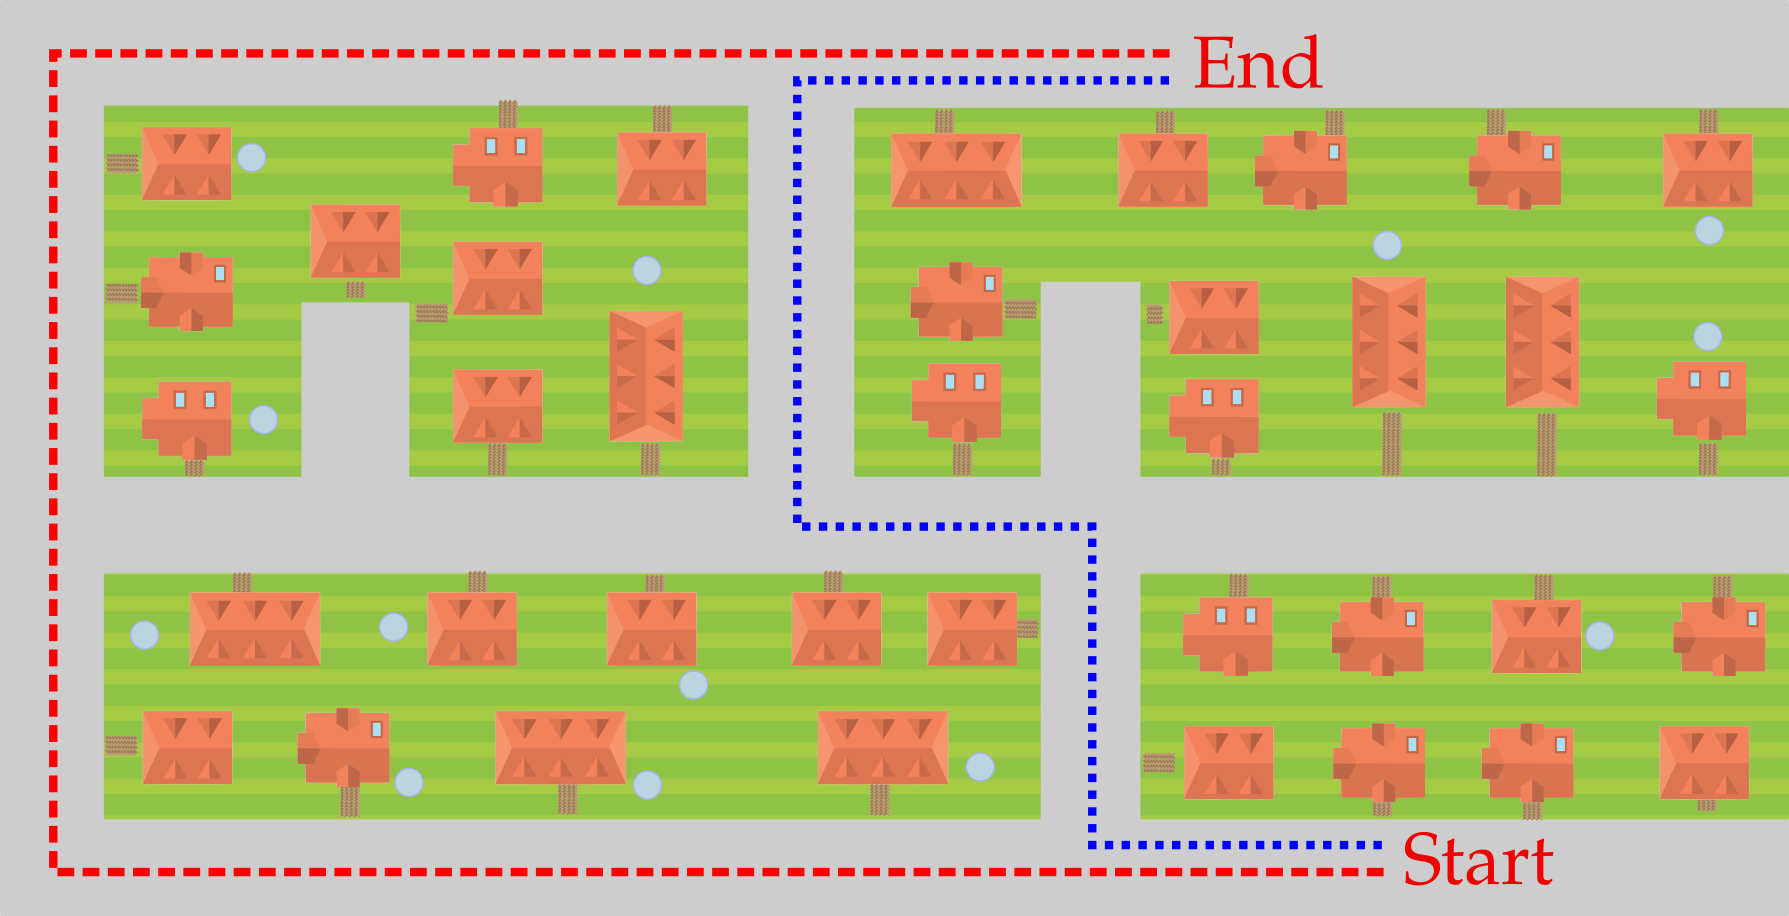
\includegraphics[scale=0.22]{figures/chapter3/landscape/landscape.png}
\caption{\label{fig:chap3_shortest} Comparison of two routes in terms of complexity and length. Even if the blue route (. . .) is the shortest many directions changing are required. Each of them is a risk for the guided person to make a mistake and be lost again. The red route (- - -), although being a bit longer, is easier to explain and to remember, and has few directions changing.}
\end{figure}

Even if the use of landmarks helps at understanding direction changing by anchoring the action to be performed, they still are a risk for the guided person to make a mistake, taking the wrong path. Where the length of the route would be an important criterion is the choice of a route, its complexity is also to be taken into account when we need to explain it. Morales in~\cite{morales_2015_building} argued that reducing the route complexity, in terms of the number of stages composing it, should be prefered to its length. This feature reduces the risk of mistake concerning the choice to make along it and also has an impact on its understanding and memorization. This criteria of minimal explanation can be compared to the Grice's Maxim of quality~\cite{grice_1975_logic}. In the example of figure~\ref{fig:chap3_shortest}, some should prefer to explain the red route rather than the blue one, even if it is longer.

Finally, to explain the same route Taylor in~\cite{taylor_1992_spatial} has noticed that a speaker can use two kinds of perspective. First, the \textit{survey} perspective trend at adopting a bird's eye view point of the environment, meaning a top view of it like as looking at a map. With this perspective, the speaker refers to the different landmarks of the route with respect to one another. They are thus referred to using terms including north-south-east-west. This perspective is opposite to the \textit{route} perspective. With such a perspective, the speaker mentally navigates along the route, making an imaginary tour of the environment. As a result, he refers to the landmarks with respect to the future guided person position along the route. The landmarks are thus referred to using terms like left, right, front, or back. In~\cite{taylor_1996_perspective}, they notice that the survey perspective is generally used for open environments whereas the route perspective is generally used in environments with already identified paths. For indoor environments, the latter should thus be preferred to facilitate route understanding and memorization.

\subsection{Environment represention to compute routes}

Regarding the environment representation generally used to find itineraries, we can first take a look to GNSS road navigation systems. In \cite{liu_1997_route} or \cite{cao_2009_gps}, we find the same principle of a topological network representing the roads with semantic information attached to each of them. Such representation seems adapted regarding the performance required for such systems operating in very large areas. However, GNSS road navigation systems must respond only to this unique task of finding a path when a robot is expected to be able to answer to various tasks. For our application, we thus need a representation that can be used more widely while still allowing the search for routes.

%Morales et al. \cite{morales_building_2015} indicate that naming parts of a geometric map does not leave the opportunity to compute such perspective. As in \cite{satake_field_2015}, we have chosen to develop our representation with an ontology as it allows to reason about the meaning of words and thus improve the understanding of human demands. In addition, we propose a way to merge the topological representation into the semantic representation (the ontology) to get the meaning of the environment elements while keeping a description of the connectivity of the elements of the environment. We propose to name it semantic spatial representation (SSR). 

% More than the extension of the spatial semantic hierarchy (SSH) \cite{kuipers_spatial_2000} allowing the representation of the environment

%This paper focuses on the presentation of the SSR and on its usability for the route description task. For now, all the ontologies used to test the SSR have been made by hand. However, many recent research work leads to automatically generate a topological representation of an environment from geometric measurements (e.g. Region Adjacency Graphs \cite{kuipers_local_2004}, Cell and Portal Graphs \cite{lefebvre_automatic_2003} or hierarchical models \cite{lorenz_hybrid_2006}, or from natural language \cite{hemachandra_learning_2014}). We have not done it yet, but our system could benefit from this work to generate a representation of an environment using SSR, which would solve the complexity of creating such a representation by hand.

\section{The Semantic Spatial Representation}

\subsection{The SSR classes}

\begin{figure}[ht!]
\centering
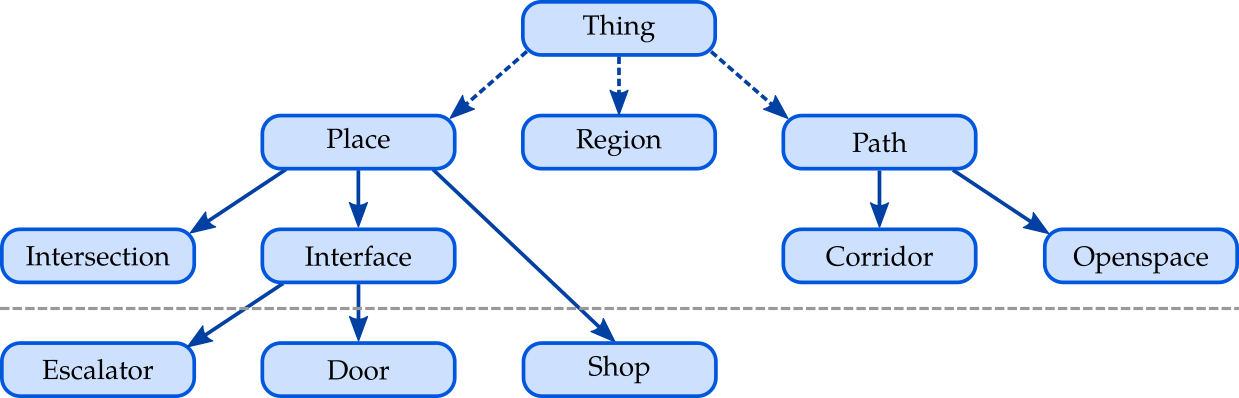
\includegraphics[scale=0.4]{figures/chapter3/ssr_tbox.png}
\caption{\label{fig:chap3_tbox} Representation fo the TBox (classes hierarchy) of the Semantic Spatial Representation used to describe the topology of an indoor environment. While the top part is inherent to the SSR, the bottom one extends the latter to provide more granularity.}
\end{figure}

\subsection{The SSR properties}

\begin{figure}[ht!]
\centering
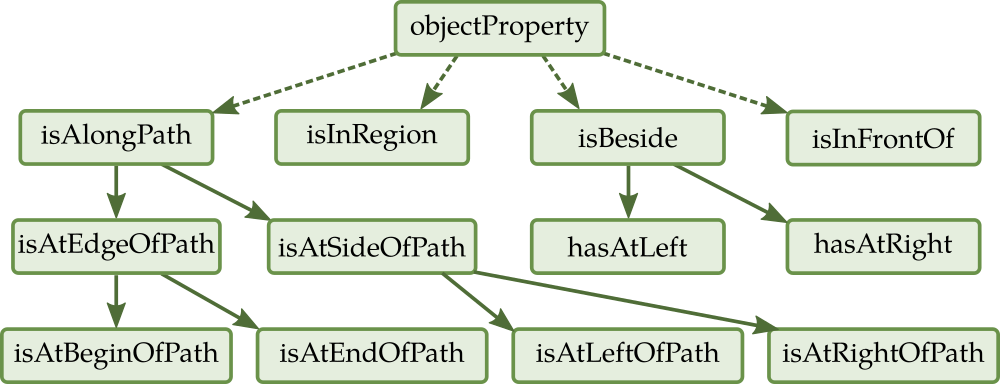
\includegraphics[scale=0.4]{figures/chapter3/ssr_rbox.png}
\caption{\label{fig:chap3_rbox} Representation fo the RBox (properties hierarchy) of the Semantic Spatial Representation used to describe the topology of an indoor environment.}
\end{figure}


\section{Finding routes to the right destination: A two-level search}

\subsection{The region-level: Trim down the search}

\begin{figure}[ht!]
\centering
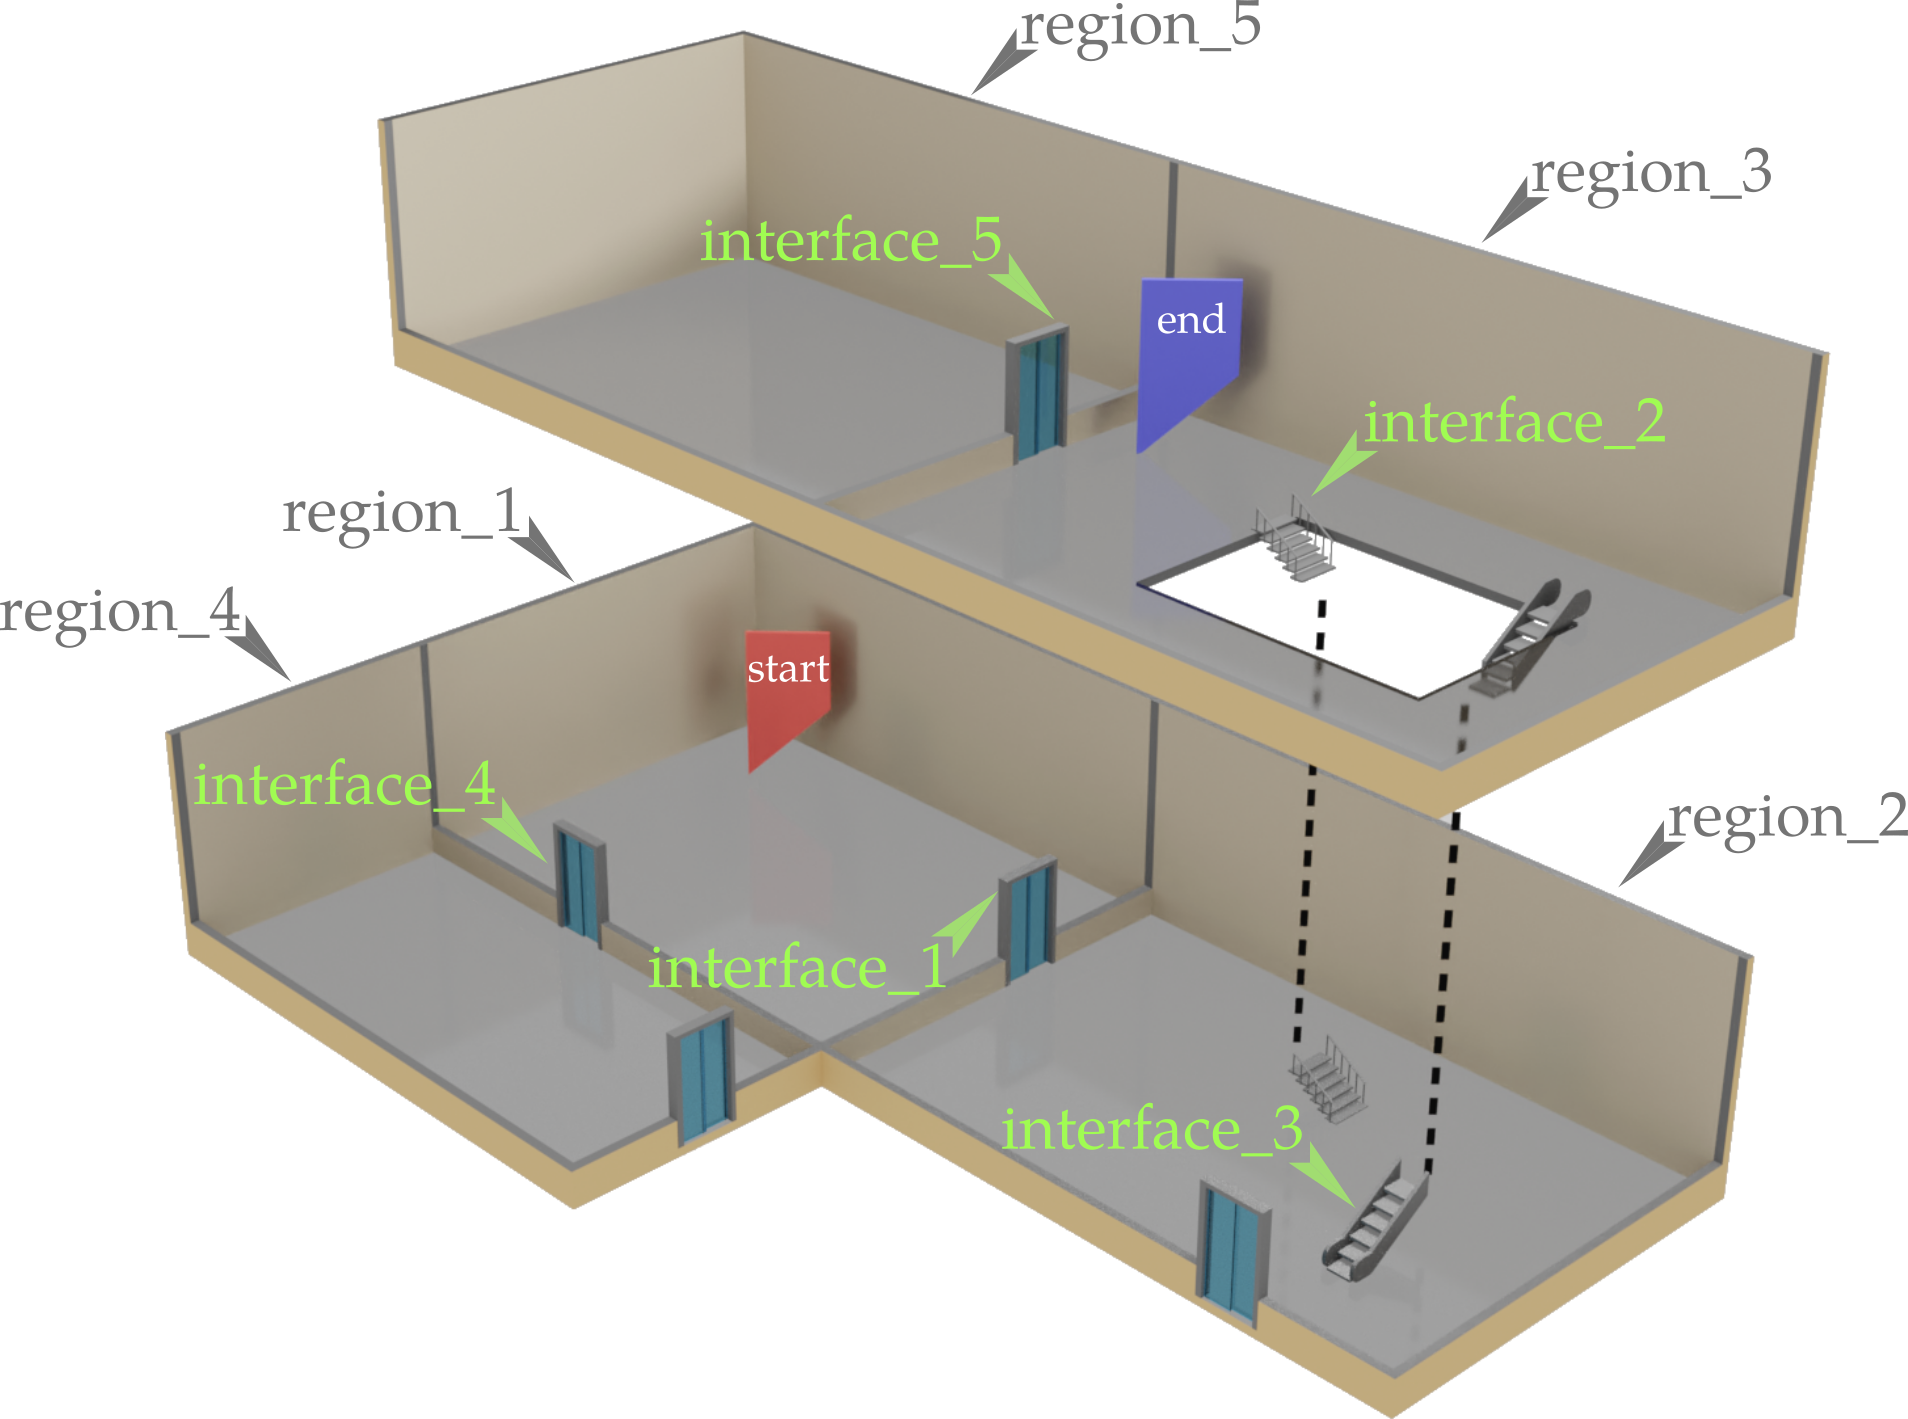
\includegraphics[scale=0.22]{figures/chapter3/building_regions.png}
\caption{\label{fig:chap3_regions} Representation of an environment at the region-level. Regions are linked trhough interfaces. We know that the starting point of the search is in \textit{region\_1} and the goal place is in \textit{region\_3}. }
\end{figure}


\subsection{The place-level: Refine the search}

\begin{figure}[ht!]
\centering
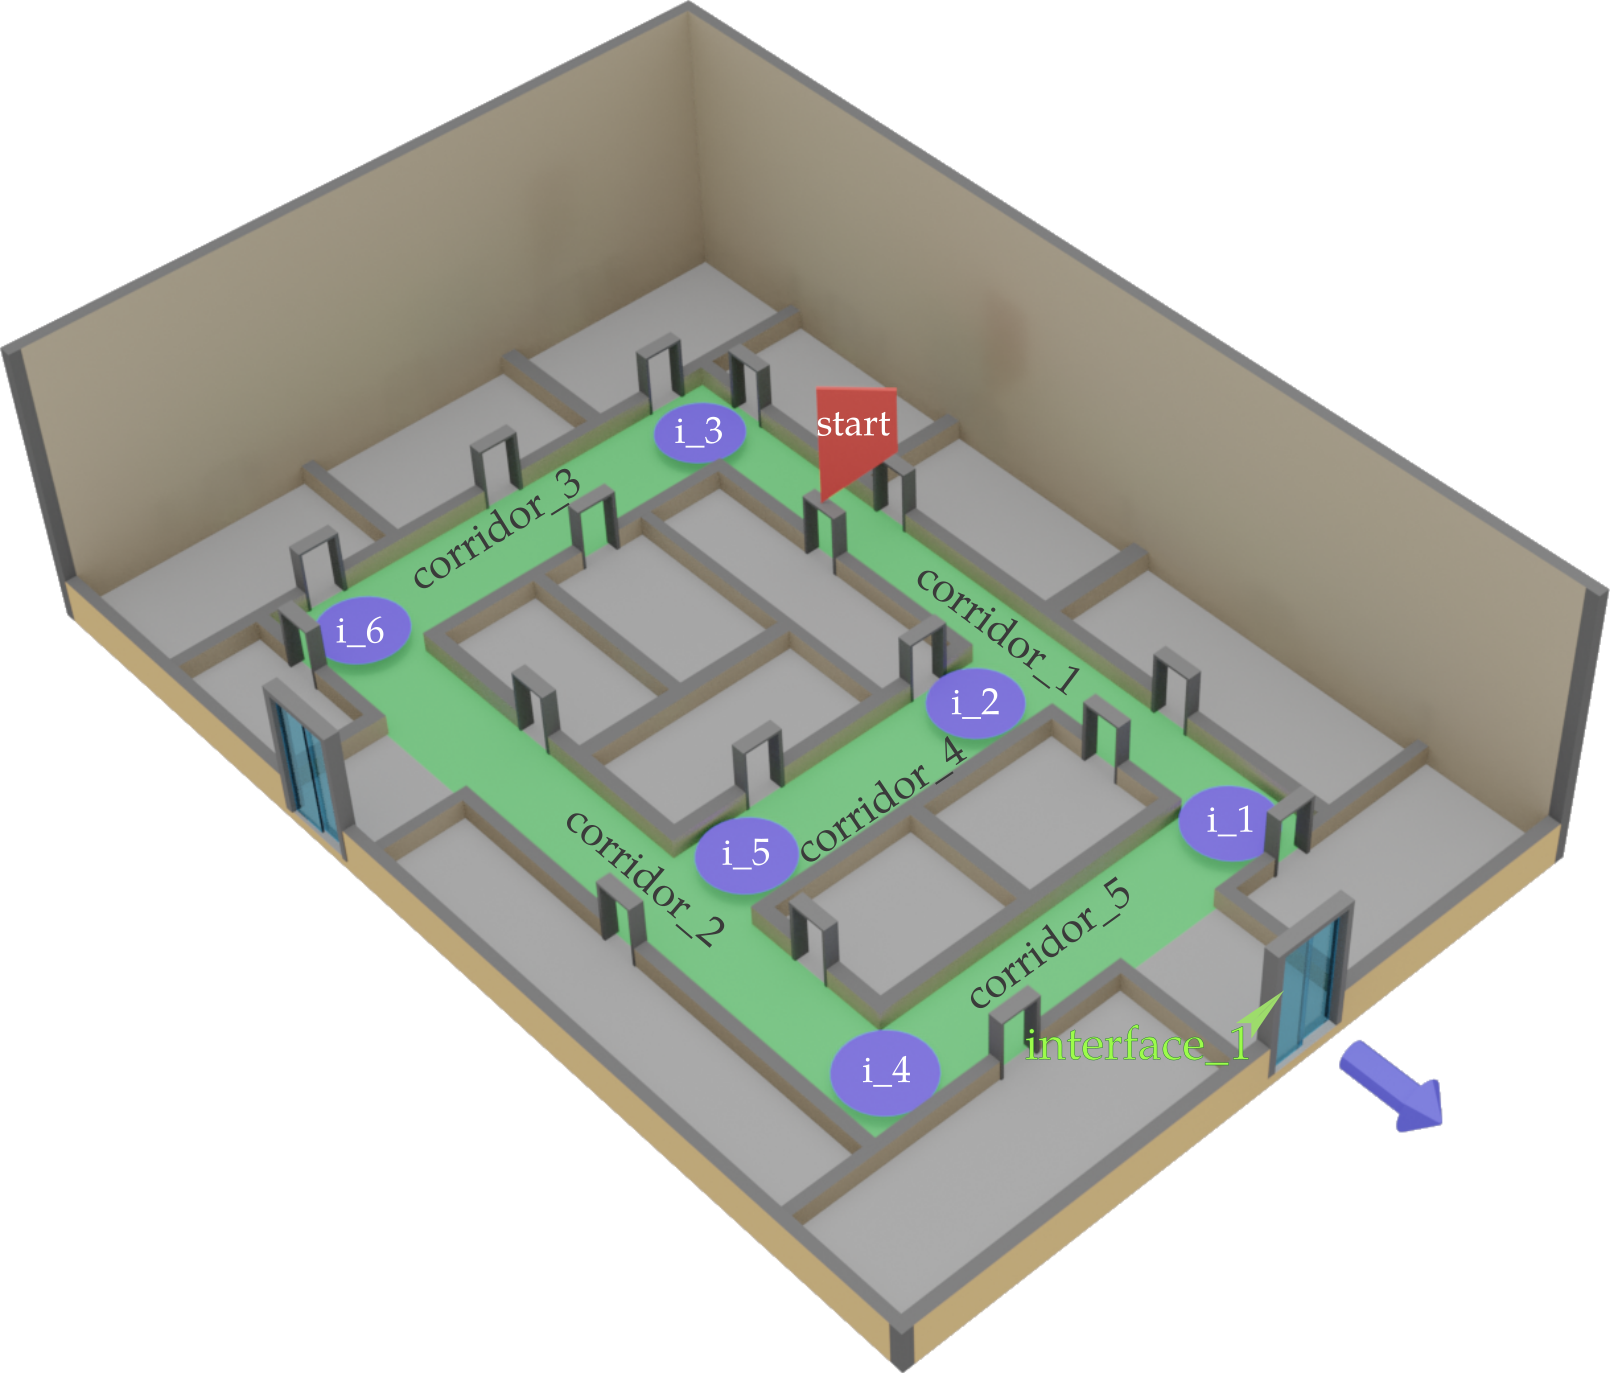
\includegraphics[scale=0.28]{figures/chapter3/region1.png}
\caption{\label{fig:chap3_region1} Representation the \textit{region\_1} at the place-level. A region is composed of paths (here corridors only) connected through intersections. We know that the starting point of the search is along \textit{corridor\_1} and the local goal place is in \textit{corridor\_5}. }
\end{figure}

\subsection{Selecting the most suitable route}

\section{Genarating an explanation in natural language}

\subsection{Putting the robot in your shoes}

\subsection{A pattern-based generation}

\section{Experiment in emulated and real environment}




\ifdefined\included
\else
\setcounter{chapter}{4} %% Numéro du chapitre précédent ;)
\dominitoc
\faketableofcontents
\fi

\chapter{Ontology-based Referring Expression Generation}
\chaptermark{Ontology-based REG}
\minitoc

The contribution presented in this chapter is excerpted from our work, published in the proceedings of the RO-MAN 2020 conference~\cite{buisan_2020_efficient}. In this manuscript, the contribution is more detailed and discussed. The presented work has been achieved in collaboration with Guilhem Buisan, with an equal contribution. Several algorithms have been developed by both of us, giving, as a result, the one presented in this chapter, merging the best of our trials. My focus was mainly on how to fully take advantage of the ontology as a knowledge base and on algorithmic optimisations to make our method the most efficient in the current literature.

\section{Introduction}

Referring to an entity is one of the most common task that we perform every day. "Can you bring me my mug? It is the black one next to the sink". "I don't remember the name of the man with the red shirt and the glasses". "I lost my keys, they are on a keychain with a soft toy in the shape of a unicorn". Such kind of communication, precise and efficient, are a key apect for the success of a collaborative tasks. Nevertheless, in complex environment with a wide variety of objects, places, or people, referring a specific entity can become a real challenge for robotic application. The robot has to take into account the context of the upper task, the diversity of facts that can be extracted from the situation and which depend on available perception modalities, and the available common ground between the robot and its partner. 

\begin{figure}[h!]
\centering
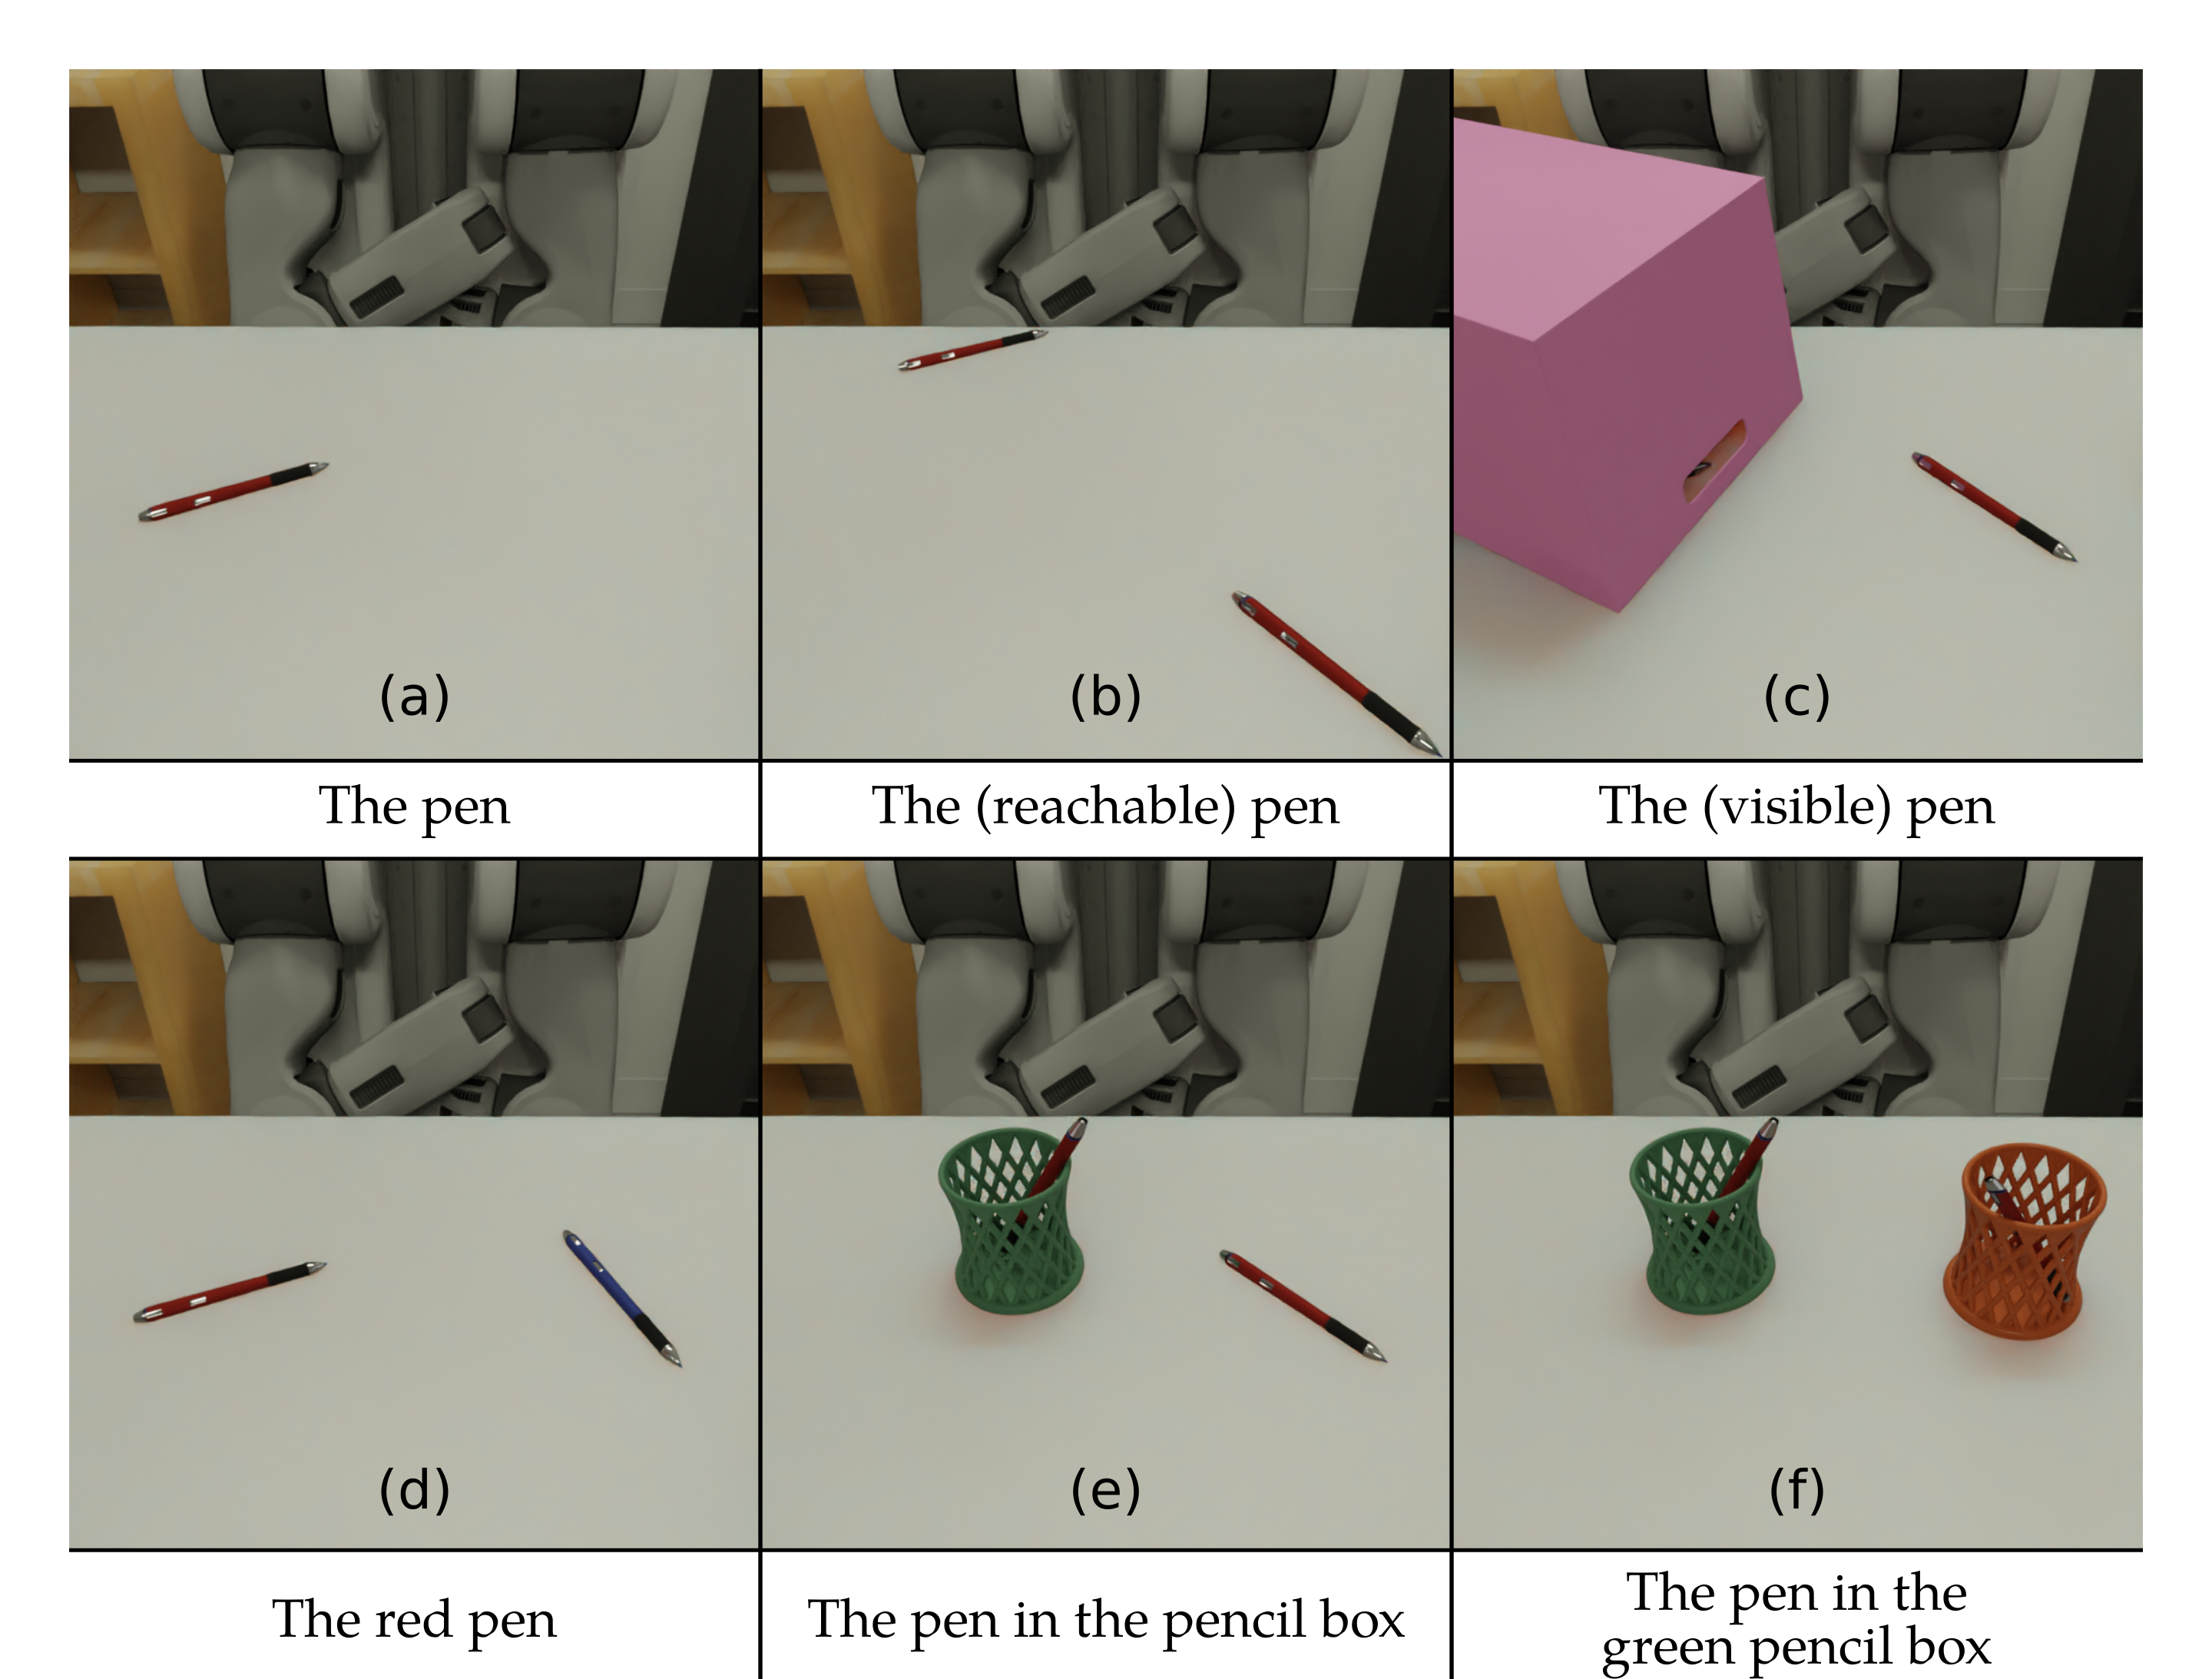
\includegraphics[scale=0.16]{figures/chapter4/intro.png}
\caption{\label{fig:chap4_intro} Six situations view from the hearer perspective, with the robot placed on the other side of the table. Referring to the same pen involves different mechanisms to raise the ambiguity, in each situation. The sentence above each situation is a possible referring expression to designate the said pen without ambiguity. }
\end{figure}

Consider the situation where you are around a table with your collaborative robot and the robot needs a pen. The simple statement \textit{"Give me the pen"} can result in several situations of different complexities. In the case where there is only one pen (Fig.\ref{fig:chap4_intro}a), the referring it is obvious. Now consider two pens on the table. If one is reachable by you (the human) and the other is not (Fig.\ref{fig:chap4_intro}b), reachability can be used to refer to the pen. If both pens are not reachable but one is visible to you and the other is not (Fig.\ref{fig:chap4_intro}c where a pen is hidden under the box), visibility through perspective-taking could be used to determine that the other pen does not lead to ambiguity. Now both pens are visible and reachable, but one is blue and the other is red (Fig.\ref{fig:chap4_intro}d). The addition of the color of the pen solves the ambiguity. If both pens have the same color but one is in a pencil box (Fig.\ref{fig:chap4_intro}e), the relation to the pencil box resolves the ambiguity. If unfortunately, both are in a pencil box but one is green and the other orange (Fig.\ref{fig:chap4_intro}f), the relation to the pencil box and the color of the latter resolves the ambiguity. We could continue like this for a long time, considering that one is at your left and one at your right, that there is no pen on the table but there is one on a shelf and so on.

Until now, we considered that the robot knows the concepts of pen and pencil box as well as their names in natural language to speak about them. However, imagine yourself travelling in another country and having to speak english\footnote{I apologize to the native English speakers who will not take full advantage of this example.}, you can sometimes miss some words and thus use more generic a one instead. However, by doing so some new ambiguity can be raised because this generic word also refers to other entities. It is the same for our robot if it has to speak French and does not know the translation of the pencil box concept. It will have to resort to a more generic term, such as "container" that can also refer to a box beside.

In addition to the concepts names, the robot must pay attention to the relationships it uses. The exact weight or length of an object wouldn't be useful as a human can not easily evaluate them. On the contrary, the color of the object seems to be a suitable property to use, unless the robot partner is color blind. This means that the robot has to use relations that it estimates to be known and observable by its partner. Such can be done considering the theory of mind and performing the generating the entity reference on the estimation by the robot of the knowledge base of the human partner.

This task to refer to a precise entity among others is commonly called the \textbf{Referring Expression Generation} (REG) task. It is often decomposed into two sub-tasks: the \textbf{content determination} and the \textbf{linguistic realisation}~\cite{krahmer_2012_computational}. The content determination aims at determining the relations to be used to refer to an entity while the linguistic realisation aims at choosing the words to be used to communicate the content. The contribution of this chapter is focused on content determination but we can not consider these two sub-tasks entirely independent. As explained earlier, if the robot does not know some concept names in natural language, the linguistic realisation will fail in the case the content determination select them or the linguistic realisation will choose a more general word that does not correspond to the determined content. We could imagine a dedicated knowledge base for the REG with only concepts usable in natural language, but such a solution is not suitable if we want a unique knowledge base for all the robotic system. Moreover, it could be hard to maintain this dedicated knowledge base during the interaction, in addition to others. 

The main contribution presented in this chapter is an \textbf{ontology-based and domain-independent algorithm for the generation of referring expressions}. It uses customizable cost function estimating the cognitive load required for a human to interpret the RE to produce \textbf{the optimal set of verbalizable assertions} that allows to refer unambiguously a given entity.

First, we review the literature concerning the REG problem and discuss the issues we aim to tackle. Then, we refine the definition of the problem to manage it at a search problem in a second part. We then compare our algorithm with two states of the art algorithms to assess its solutions and its performance. We end this chapter with integration on a real robotic system with some detail on the used perception system and the verbalization method.

\section{Related work}

Referring Expression Generation is a today classic task in Natural Language Generation \cite{gatt_2018_survey} that has been studied for decades. It has been defined by Reiter as the concern of "how we produce a description of an entity that enables the hearer to identify that entity in a given context"~\cite{reiter_2000_building}. Over time, the criteria for a good Referring Expression (RE) have been refined but still take their roots from the Grice's maxims~\cite{grice_1975_logic}. The maxim of \textit{manner} requires the communication to be unambiguous. It is also the referential success for the target entity to be unambiguously identified by the RE hearer. The maxim of \textit{relation} requires the communication to be relevant regarding the current context both the context of the task to achieve and the current world state. If you are asking someone to give you an object that is in the room where you are, you can reasonably assume that the objects in the rest of the house are not ambiguous with the one you are requesting. The maxim of \textit{quality} seems to be evident and requires the communication to be true. If you are asking a bootle and you do not know if it is full or not, you should not use this information to refer to the bottle. Finally, the maxim of \textit{quantity} requires the communication to be as informative as required but not more informative than required. In simple words, to be brief. In the context of REG, the hearer must understand quickly want you are talking about. Moreover, giving unnecessary information could lead to false implications. Saying "give me the red pen" could imply that at least one other non-red pen exists and such warn the hearer to not do the mistake to take the wrong one. If no other pen exists regarding the current context, the sentence "give me the pen" is thus sufficient.

Dale and Reiter are considered as being the pioneers of the Referring Expression Generation and have proposed over years three main algorithms solving it. Two first two fundamental approaches are the Depth First Search (DFS)~\cite{dale_1989_cooking} and the Full Brevity~\cite{dale_1992_generating}. While the first algorithm does not always find an optimal solution in terms of the number of relations used, the second does it at the cost of an exhaustive search. The most notable advance was thus the Incremental Algorithm (IA) first presented in~\cite{reiter_1992_fast} then refine in~\cite{dale_1995_computational}. With this algorithm, the notion of preference over features has been highlighted. This notion aims at representing the fact that some features are easier to understand than others. For example, the color or the shape of an object is easier the understand than spatial relations. However, the major limitation of the presented algorithms is the used knowledge representation. Because they used a set of attribute-value pairs for each entity, the solutions can only be composed of entity attributes and cannot use relations between entities. To be more precise, the algorithms can give the fact the referred entity is on a table but cannot discriminate the said table among others.

With the introduction of a new representation in the form of a labeled directed multi-graph (also known as the REG graph), Krahmer et al. solved the issue of the reference to other entities~\cite{krahmer_2003_graph}. The related Graph-Based Algorithm (GBA) REG is able to manage relations between entities and, as Dale and Reiter, consider a preference over features. This preference, called Preference Ordering (PO), is represented by a cost assigned to each edge of the graph. The GBA algorithm uses a branch\&bound algorithm which allows finding the optimal RE. On this new basis, extensions have been developed or at least discussed. Regarding the thin link with Description Logic, Krahmer raised the problem of the hierarchy of entity types in~\cite{krahmer_2012_computational}. On its side, Li et al. have proposed an optimized version of the GBA~\cite{li_2017_automatically} GBA allowing an efficiency gain close to 56\%. However, the used task only involved cubes, meaning that their algorithm does not have to take into account the entities' types, which were just added as a post-process. A last interesting GBA is the Longest First (LF) algorithm presented in~\cite{viethen_2013_graphs}. However, more than not respecting the maxim of quantity, its exhaustive search entails poor performance when used on larger realistic knowledge bases.

Learning-based approaches have of course been proposed. The belief network-based method presented in~\cite{yamakata_2004_belief} can only work with objects' attributes. Moreover, the authors indicate that a specific belief network should be constructed and therefore trained for each attribute. Such limitation reduces the genericity of the method. With a log-linear model trained from a corpus of the probability distribution of REs~\cite{fitzgerald_2013_learning}, Fitzgerald et al. face the same problem. Nevertheless, by working on belief bases, Yamakata has highlighted the importance to run the algorithm on the human partner's estimated belief base. It ensures the robot generates a referring solution compatible with concepts estimated to be known by the human.

All the algorithms presented here before are highly dependent on the task to perform. Where learning approaches are dependent on their training corpus, the other relies on knowledge bases integrating only relations usable in the context of the task. Williams et al. proposed a hybrid approach between domain-dependent and domain-independent with a distributed Incremental Algorithm (DIST-PIA)~\cite{williams_2017_referring}. The idea besides this algorithm is to make the core Incremental Algorithm independent of the knowledge representation by making it querying domain-dependent consultants~\cite{williams_2016_framework}. A consultant is an interface of a knowledge base and each knowledge base of the distributed architecture owns one. Each consultant is thus dedicated to a specific set of properties and can be query regarding these properties. To get relations about the location of entities, the Incremental Algorithm can thus query the consultant associated with the knowledge base of locations. While this solution is interesting for distributed architectures, we can ask ourselves about the domain-independence of the core Incremental Algorithm. Indeed, the ordering of the consultants to query in the algorithm can have an impact on the found solution. However, it is worth mentioning that this method has been successfully integrated into a robotic architecture~\cite{williams_2019_dempster}.

At the date, the closest work to the one presented in this chapter is introduced in~\cite{ros_2010_which}. This method uses ontology as a knowledge base. As explained earlier, such knowledge representation is suitable for domain-independent applications. However, here again, the used algorithm takes as a hypothesis that only relations useful for the REG task are present in it. Moreover, in the same way as the IA-based algorithm, their method only supports entities' attributes and not relations between entities. This method has still been integrated into a robotic system that can take advantage of perspective-taking to construct an estimated knowledge base of the human partner to give pertinent RE~\cite{lemaignan_2011_grounding}.

Even if all the presented algorithms rely on different kinds of knowledge representation and have non-equivalent abilities, they all consider a perfect linguistic realisation~\cite{krahmer_2012_computational}. We mean here that they all consider that any concept of their knowledge bases has a word in natural language and can thus be verbalize. Wanting to run on the same knowledge base as the other component of the robotic architecture, we do not want to make this assumption. Even if our contribution is focused on content determination, we aim with this contribution to make a first step in the linguistic realisation by not considering these to sub-task as being independent of one the other. We thus assume that not all the concepts in the knowledge base can be used in natural language.

To give a better overview of the progress in the REG field, the most representative contributions presented above are summarized in Table.~\ref{tab:reg_ref_sumup}. The contributions are organized chronologically and around six major features that we have mentioned throughout this section. These desired features are:
\begin{itemize}
	\item \textbf{Domain independent}: The knowledge base used by the REG must be able to be used by other components of a robotic architecture. The REG algorithm must not consider that all the knowledge represented can be used for this task.
	\item \textbf{Representation type}: The used knowledge representation must be able to be updated all along an interaction to deal with the dynamic of robotic applications.
	\item \textbf{Use of types}: The type of an entity is the minimal information to use to refer to an entity. Without type, linguistic realisation can not be done.
	\item \textbf{Preference ordering (PO)}: Some properties are easier to understand than others. Ordering the properties according to this preference allows finding efficient referring expressions.
	\item \textbf{Referring to other entities}: Entities attributes are not sufficient to find referring expressions in realistic situations. Being able to refer to an entity by referring to another one is thus mandatory.
	\item \textbf{Natural language}: Considering the linguistic realisation during the content generation could prevent the appearance of ambiguity at the linguistic realisation or even the incapacity to perform it.
\end{itemize}

\begin{table}[!h]
\centering
\caption{Summary of the most representative contributions in the REG field regarding the six major features of the problem. The contributions are listed in chronological order to give a better overview of progress in the field.}
\label{tab:reg_ref_sumup}
\begin{tabular}{lcccccc}
\hline
\multicolumn{1}{|c|}{Contributions} & \multicolumn{1}{c|}{\begin{tabular}[c]{@{}c@{}}Domain\\ inde-\\ pendent\end{tabular}} & \multicolumn{1}{c|}{\begin{tabular}[c]{@{}c@{}}Rep.\\ Type\end{tabular}} & \multicolumn{1}{c|}{\begin{tabular}[c]{@{}c@{}}Use of\\ types\end{tabular}} & \multicolumn{1}{c|}{PO}  & \multicolumn{1}{c|}{\begin{tabular}[c]{@{}c@{}}Referring\\ to other\\ entities\end{tabular}} & \multicolumn{1}{c|}{\begin{tabular}[c]{@{}c@{}}Natural\\ language\end{tabular}} \\ [0.5ex] \hline \hline
\cite{dale_1989_cooking}            & \cellcolor{red!25} No                                                                 & \begin{tabular}[c]{@{}c@{}}Knowledge\\ base entity\end{tabular}          & \cellcolor{red!25} No                                                       & \cellcolor{red!25} No    & \cellcolor{red!25} No                                                                        & \cellcolor{red!25} No                                                           \\
\cite{dale_1992_generating}         & \cellcolor{red!25} No                                                                 & -                                                                        & -                                                                           & \cellcolor{red!25} No    & \cellcolor{red!25} No                                                                        & \cellcolor{red!25} No                                                           \\
\cite{reiter_1992_fast}             & \cellcolor{red!25} No                                                                 & \begin{tabular}[c]{@{}c@{}}attribute-\\ value pairs\end{tabular}         & \cellcolor{green!25} Yes                                                    & \cellcolor{green!25} Yes & \cellcolor{red!25} No                                                                        & \cellcolor{red!25} No                                                           \\
\cite{krahmer_2003_graph}           & \cellcolor{red!25} No                                                                 & REG graph                                                                & \cellcolor{red!25} No                                                       & \cellcolor{green!25} Yes & \cellcolor{green!25} Yes                                                                     & \cellcolor{red!25} No                                                           \\
\cite{yamakata_2004_belief}         & \cellcolor{red!25} No                                                                 & \begin{tabular}[c]{@{}c@{}}Belief\\ Network\end{tabular}                 & \cellcolor{red!25} No                                                       & \cellcolor{green!25} Yes & \cellcolor{red!25} No                                                                        & \cellcolor{red!25} No                                                           \\
\cite{ros_2010_which}               & \cellcolor{orange!25} Yes                                                             & Ontology                                                                 & \cellcolor{red!25} No                                                       & \cellcolor{green!25} Yes & \cellcolor{red!25} No                                                                        & \cellcolor{red!25} No                                                           \\
\cite{viethen_2013_graphs}          & \cellcolor{red!25} No                                                                 & REG graph                                                                & \cellcolor{red!25} No                                                       & \cellcolor{green!25} Yes & \cellcolor{green!25} Yes                                                                     & \cellcolor{red!25} No                                                           \\
\cite{williams_2017_referring}      & \cellcolor{orange!25} Yes                                                             & \begin{tabular}[c]{@{}c@{}}Distributed\\ KBs\end{tabular}                & \cellcolor{red!25} No                                                       & \cellcolor{green!25} Yes & \cellcolor{red!25} No                                                                        & \cellcolor{red!25} No                                                           \\
\cite{buisan_2020_efficient}        & \cellcolor{green!25} Yes                                                              & Ontology                                                                 & \cellcolor{green!25} Yes                                                    & \cellcolor{green!25} Yes & \cellcolor{green!25} Yes                                                                     & \cellcolor{green!25} Yes                                                       
\end{tabular}
\end{table}

The literature presented here before is focused on Referring Expression Generation in its nominal form. Some researches have however addressed side problems that we do not aim to tackle. Not entering much in the details, we mention them to give a more global picture of the field. The use of spatial relations is not trivial as these relations can differ for certain entities taking the RE emitter's or receiver's point of view while for other entities, having a clear orientation system (e.g. a car), the relations remain unchanged~\cite{kelleher_2006_incremental, dos_2015_generating}. Spatial relations can also be expressed not only based on a single entity but also according to a set of entity~\cite{fang_2013_towards}. While a RE is often considered as being a single sentence referring to an entity without ambiguity, some see it as a more collaborative task where the RE is provided step by step, allowing to catch acknowledgement and to refine it according to the receiver comprehension~\cite{fang_2014_collaborative, wallbridge_2019_generating}. Finally, some research tries to integrate REG in a more global interaction where several agents refer to entities. The robot thus tries to reuse properties previously used by the partner ensuring that these properties are known~\cite{williams_2020_toward}. Limitations about this work will be discussed later in this thesis.

\section{Define the REG problem}

In this section, we present the ontology of example that we use all along with this chapter. We then discuss how the up-task in which a REG could be performed can restrict the search among the entire knowledge base. Finally, we formally define the expected form for a solution to a REG problem and the constraints it must respect.


\subsection{The knowledge representation}
\label{sec:chap4_kb}

As presented earlier in this thesis, ontology is a way to represente knowledge that is now largely used in many field becasue it allows a standardization of the representation easy extension of an extisting knowledge base, and the use of inference engine to enrich the the knowledge base. For these reasons, we choose to use a knowledge base in the form of an ontology as input of our algorithm for the REG problem. Moreover, we saw that number of recent REG algorithm have trend to use graph representations as it allows to refer to an entity through relations to other entities. Because an ontology can be see as a more complexe and mor expressive graph, this representation seems to be adequate to use for the REG problem. 

\begin{figure}[h!]
\centering
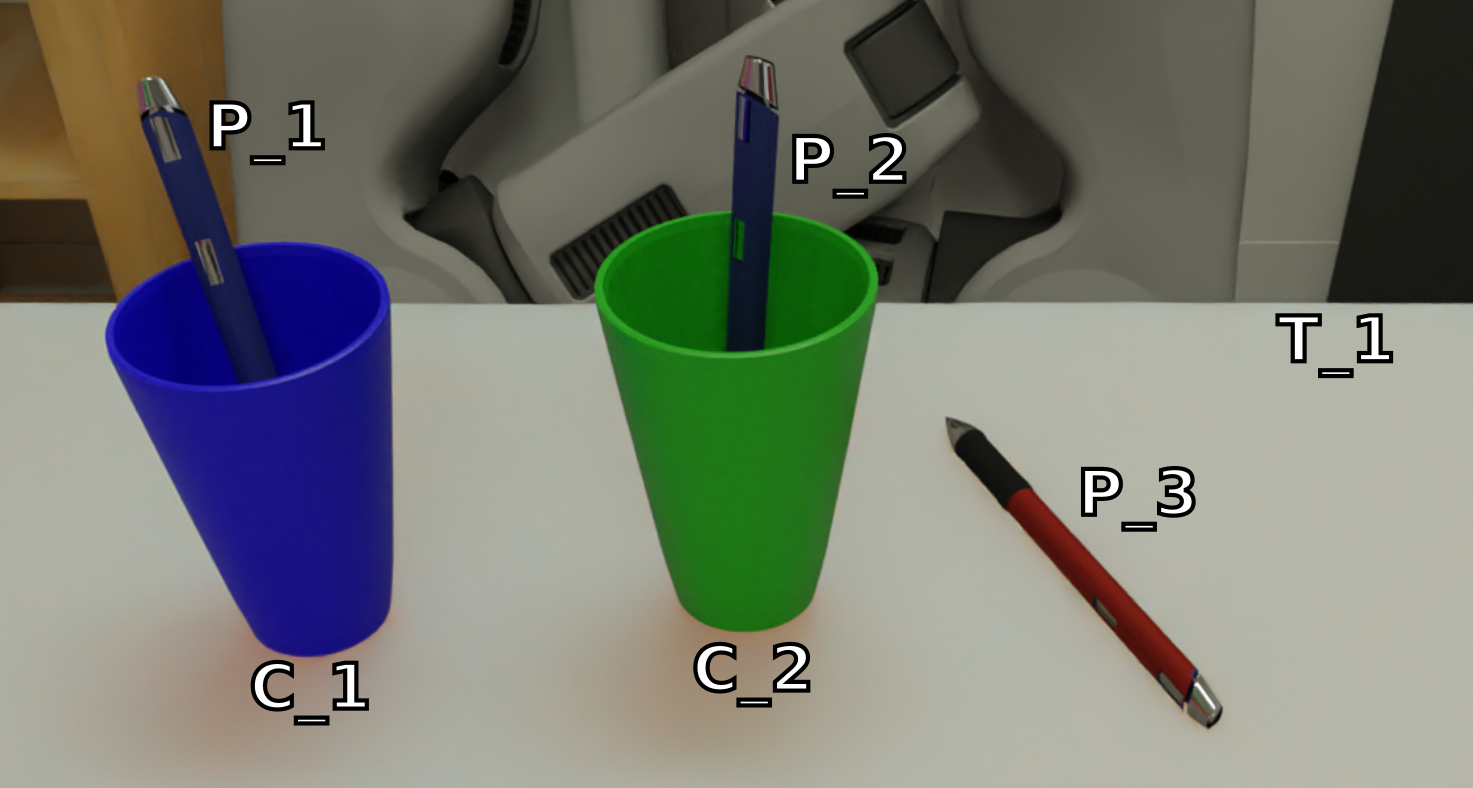
\includegraphics[scale=0.2]{figures/chapter4/pens.png}
\caption{\label{fig:chap4_kb} A situation view from the hearer perspective, with the robot placed on the other side of the table. Three pens and two cups are on a table. The two blue pens are each in one cup. }
\end{figure}

In this chapter, we take as an example the situation represented in Figure~\ref{fig:chap4_kb}. The situation is assumed to be perceived by the robot and represented in its semantic knowledge base. This knowledge base as an ontology is of the form $\kbs^R = \langle \Abox^R, \Tbox^R, \Rbox^R \rangle$. $\Abox$, $\Tbox$ like presented in Section~\ref{sec:kb_formalism}. The estimated knowledge base of the human partner $\kbs^H$ is here assumed to be the same as that of the robot in the way that $\kbs^R \equiv \kbs^H \equiv \kbs$.

The Tbox used to describe the situation of example is represented in Figure~\ref{fig:chap4_kb_Tbox}. The class IkeaLisabo represent a precise model of tables and does not have any label. The class Pen is specified through two classes the ClickingPen and the TurningPen. These two classes aim at representing the pens you need to click on top to get the tip of the pen out and the pens you need to turn to get the tip of the pen out. These classes do not have any label to directly speak about them. They are such used for the robot to know how to use them. For sure a more precise ontology could be drawn but we try to keep it simple for the purpose of this chapter.

\begin{figure}[h!]
\centering
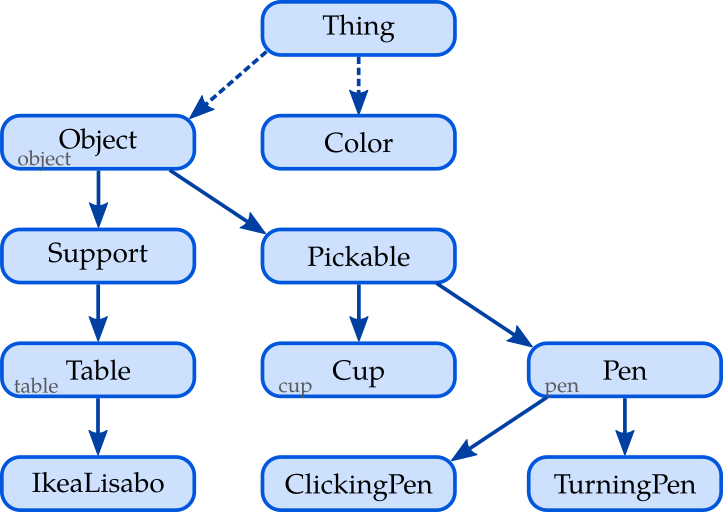
\includegraphics[scale=0.4]{figures/chapter4/pens_Tbox.png}
\caption{\label{fig:chap4_kb_Tbox} Representation of the Tbox (classes hierarchy) used to describe the situation of the Figure~\ref{fig:chap4_kb}. }
\end{figure}

The Abox used to describe the situation is represented in Figure~\ref{fig:chap4_kb_Abox}. The two cups C\_1 and C\_2 are on the table T\_1. The two pens P\_1 and P\_2 are respectivly in the cups C\_1 and C\_2 while P\_3 is directly on the table. The pen P\_4 is another pen, not on the table. Other objects could be represented as the robot and the human could know other object being in the room. the pen P\_1 is the only pen for which the agent has to click to get the tip of the pen out.

\begin{figure}[h!]
\centering
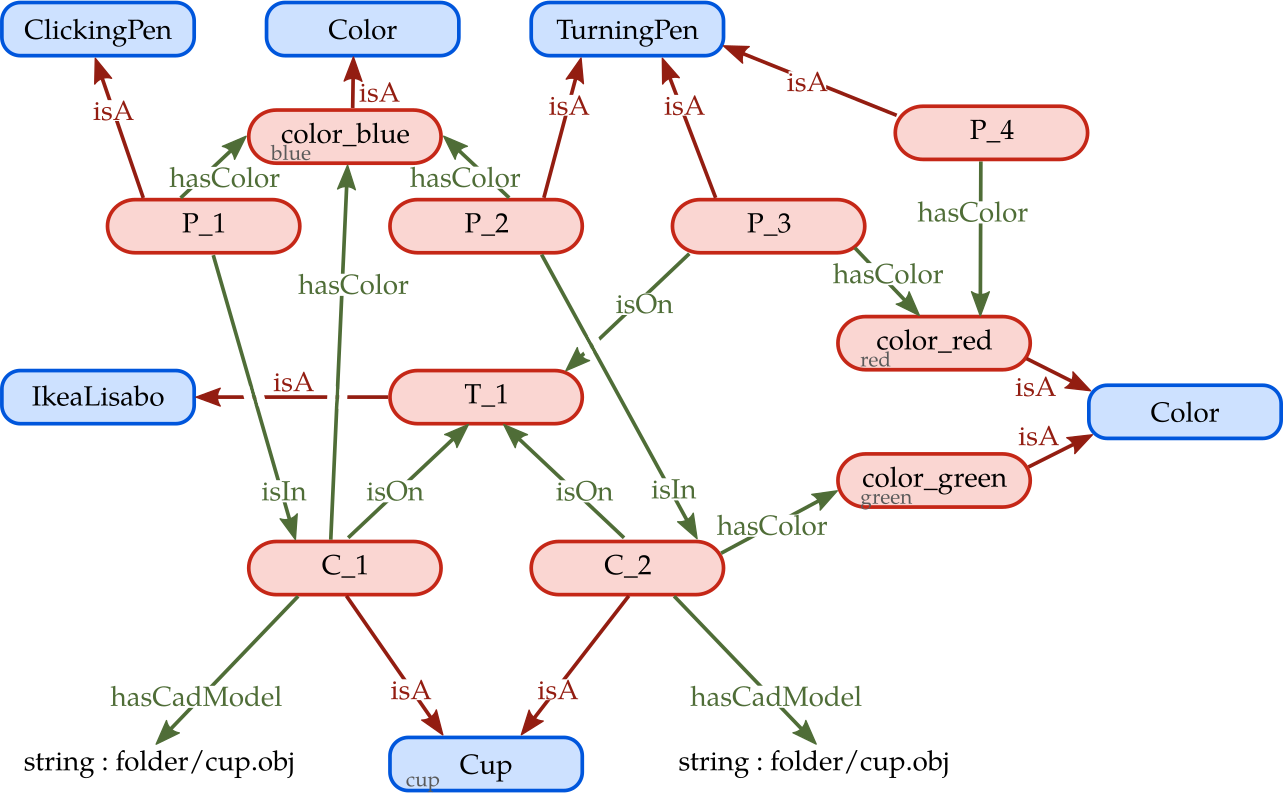
\includegraphics[scale=0.38]{figures/chapter4/pens_Abox.png}
\caption{\label{fig:chap4_kb_Abox} Representation of the Abox (relation graph) used to describe the situation of the Figure~\ref{fig:chap4_kb}. }
\end{figure}

The Rbox is not represented but the properties composing it are the ones used in the Abox. In addition with define the properties \textit{hasIn} being the inverse of \textit{isIn} and \textit{isUnder} being the inverse of \textit{isOn} ($\{(isIn,\ hasIn), (isOn,\ isUnder)\} \subset \invset$). Moreover, the property \textit{isOn} inherits of the upper property \textit{isAbove} ($\{(isOn,\ isABove), (isUnder,\ isBelow)\} \subset \inclset$). While the first state a direct contact between two entities, the other does not. Finally, we declare the chain axiom: $isIn \bullet isOn \Rightarrow isABove$. This axiom allows to reason on the ontology and declare that if an first entity is in a second one and that this second is on a third one, the first entity is above the third. Taking our example, because P\_1 is in C\_1 that is on T\_1, the pen P\_1 is above the table T\_1.


\subsection{Contextualization and restriction for situated REG}

The human (named Tony) and the robot are involved in a shared task around a table. During the task, the robot needs a blue pen to write. However, It can not take one by itself as the blue pens are on cups. Moreover, with its huge gripper, it can not use the kind of pens where you have to click. Our robot thus precisely need the pen P\_2 of our example and has to ask it to its human partner\footnote{Some could tell that if it is not the first time that our robot and this human collaborate, the human could be aware of the robot capabilities. In this case, the robot would just have to ask for a blue pen and the task would be over. We thus consider that our robot never had interacted with this particular human. For sure it could explain its capabilities but the purpose is not there.}.

The robot is thus aiming to unambiguously designate a specific entity $\goalindiv \in \indivset$, called the \textbf{target entity}, through its attributes and relations to other entities. However, as explained, the REG is meant to be used in the context of an upper task that has to be taken into account. In our example, the collaborative task concerns object on the table so that the other entities in the room are clearly out of context. Asking for a pen, P\_4 will not lead to an ambiguous situation as it is not on the table around which the interaction is performed. To represent this restriction, we provide the problem a \textbf{context} $Ctx = (\relationset_{ctx}, \inheritset_{ctx})$. It is a set of relations and direct types that are implicit in the current communication with regard to the task. This context is used to find a reference to $\goalindiv$, but has not to be included in the generated RE. For our example the context could be $Ctx = (\{ (\goalindiv,\ isAbove,\ T\_1), (\goalindiv,\ isVisibleBy,\ Tony) \},\ \emptyset)$. With this context, we state that the entity to refer to (i.e. $\goalindiv$) is known to be above the table T\_1 and visible by the human partner, Tony. Because $isAbove$ is an upper property of $isOn$, all entities on the table are concerned. Moreover, thanks to the chain axiom, any entity being in an entity on the table are also concerned. The direct types in the context could be used in a more complex communication in which we already know that we are speaking about a pen.

In addition to the entities being out of the context and thus not taken into account, some relations might be present in the knowledge base, but cannot be used in a communication process. In our example, the relations using the \textit{hasCadModel} property should not be used as the robot cannot communicate them verbally. To represent this restriction, we provide the problem a set of so-called \mbox{\textbf{usable properties}} $\usablepropset \subseteq \propset$. Any relation involving as predicate a property that is not part of the usable properties set can, therefore, not be used in the solution. Because of properties inheritance, $Incl$ all the properties inheriting from the ones in $\usablepropset$ are consequently usable to solve the problem. 


With regard to the presented restrictions, the REG problem is define as follow:

\begin{definition}[Referring Expression Generation problem]
The REG problem is a tuple $\problem = \langle \goalindiv, \kb, Ctx, \usablepropset \rangle$ with $\goalindiv \in \indivset$ the target entity, $\kbs$ the hearer semantic knowledge base, $Ctx$ the RE context, and $\usablepropset \in \propset$ the usable properties.
\end{definition}

A representation of the Abox on which the restrictions have been applied\footnote{We do not create a second Abox with the only elements that can be used. The REG algorithm will have to manage the restrictions during the search process. Otherwise, we lost the interest to run on a knowledge base common to the entire robotic architecture.} is represented in Figure~\ref{fig:chap4_kb_ctx}.

\begin{figure}[h!]
\centering
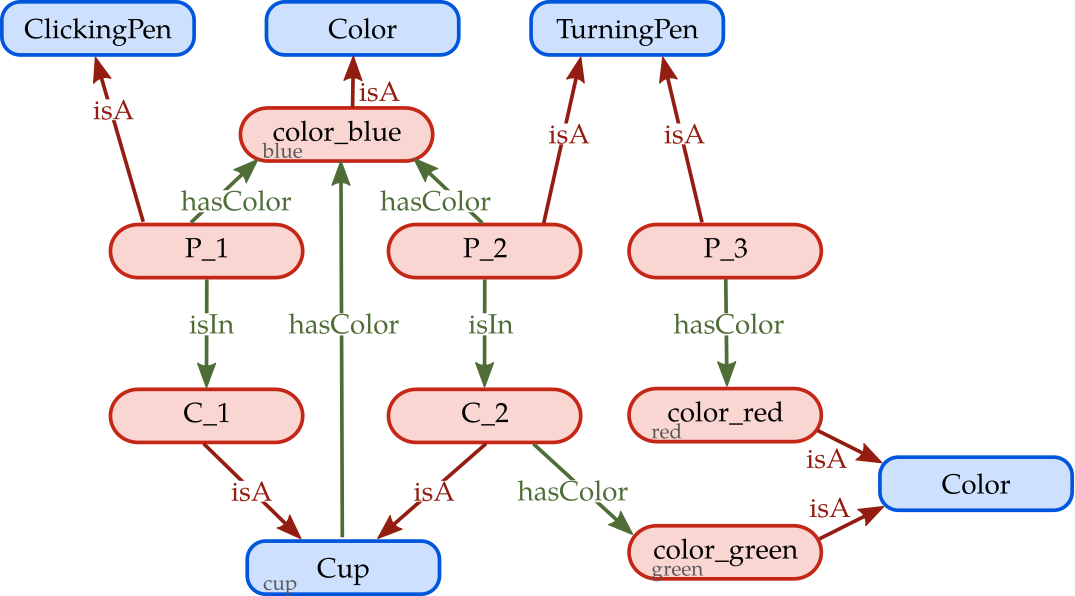
\includegraphics[scale=0.38]{figures/chapter4/pens_ctx.png}
\caption{\label{fig:chap4_kb_ctx} Representation of the Abox (relation graph) on which the context of the problem and the usable properties have been applied. }
\end{figure}

\subsection{Expected solution: structure and validity criteria}

What we could expect from a REG solver, would be a sentence in natural language. However, as explained earlier, we focus here on the sub-task that is the content generation rather than the linguistic realization. For the content generation, the attempted solution as thus often be a set of relations like $\{ (\goalindiv,\ hasColor,\ red)\}$. The issue of such a set is that it can not be verbalized afterwards. Indeed, some entities are not labelled and thus can not be used directly in the solution. They are what we called \textbf{anonymous entities}. To refer to an anonymous entity and be able to speak about it we must pass at least by its type. This is what we naturally do when we say \textit{"the red pen"} where the concept \textit{"pen"} does not directly refer to the entity by to its type. Before going ahead in the definition of the form of the solution, we can already set a constraint on its content through \textbf{the parlance need}.

\begin{theorem} [The parlance need]
\label{the:parlance_need}
For any entity appearing in a RE, exactly one naming relation must be added.
\end{theorem}

What we call a naming relation is in its simplest form the presence of a label. The relation to add is thus of the form: $(\indiv_t,\ hasLabel,\ "tony")$. In the case an entity does not have any label, we pass by one of its type which has a label: $\{(\indiv_t,\ isA,\ Pen), (Pen,\ hasLabel,\ "pen")\}$. This type is not necessarily the direct type of an entity. It could be an inherited one if needed.

Let us now introduce $\varset$, a set of variables. Because anonymous entities are not directly present in the RE sentence (hence the presence of ambiguities), we will replace all of them with variables prefixed with a question mark. The set $\varset$ thus keep a track of these variables. Taking the example of the red pen the set of relation become: \textit{\{(?0, isA, Pen), (Pen, hasLabel, "pen"), (?0, hasColor, red), (red,  hasLabel, "red")\}}. Because anonymous entities are now represented by variables, the relations representing the labels can be removed as it is implicit that the others have one. The reference is thus \textit{\{(?0, isA, Pen), (?0, hasColor, red)\}} that is exactly of the form of a \sparql{} query.

\begin{table}[b!]
\resizebox{\textwidth}{!}{%
\begin{tabular}{|l|l|l|l|l|l|}
\hline
 &
  \textbf{Target} &
  \textbf{Relations set} &
  \textbf{sparql query} &
  \textbf{Sentence} &
  \textbf{Instantiations} \\ \hline
a) &
  P\_3 &
  \begin{tabular}[c]{@{}l@{}}\{(P\_3, isA, Pen),\\ (P\_3, hasColor, red)\}\end{tabular} &
  \begin{tabular}[c]{@{}l@{}}\{(?0, isA, Pen),\\ (?0, hasColor, red)\}\end{tabular} &
  The red pen &
  {[}?0 =\textgreater P\_3{]} \\ \hline
b) &
  P\_2 &
  \begin{tabular}[c]{@{}l@{}}\{(P\_2, isA, Pen),\\ (P\_2, isIn, C\_2)\\ (C\_2, isA, Cup)\}\end{tabular} &
  \begin{tabular}[c]{@{}l@{}}\{(?0, isA, Pen),\\ (?0, isIn, ?1)\\ (?1, isA, Cup)\}\end{tabular} &
  \begin{tabular}[c]{@{}l@{}}The pen in\\ the cup\end{tabular} &
  \begin{tabular}[c]{@{}l@{}}{[}?0 =\textgreater P\_2,\\ ?1 =\textgreater C\_2{]},\\ {[}?0 =\textgreater P\_1,\\ ?1 =\textgreater C\_1{]}\end{tabular} \\ \hline
c) &
  P\_2 &
  \begin{tabular}[c]{@{}l@{}}\{(P\_2, isA, Pen),\\ (P\_2, isIn, C\_2),\\ (C\_2, isA, Cup),\\ (C\_2, hasColor, green)\}\end{tabular} &
  \begin{tabular}[c]{@{}l@{}}\{(?0, isA, Pen),\\ (?0, isIn, ?1),\\ (?1, isA, Cup),\\ (?1, hasColor, green)\}\end{tabular} &
  \begin{tabular}[c]{@{}l@{}}The pen in\\ the green cup\end{tabular} &
  \begin{tabular}[c]{@{}l@{}}{[}?0 =\textgreater P\_2,\\ ?1 =\textgreater C\_2{]}\end{tabular} \\ \hline
\end{tabular}%
}
\caption{Three referring expressions extracted from the example of Fig.~\ref{fig:chap4_intro}. For each target, is represented the relations set, the equivalent \sparql{} query, the corresponding sentence in natural language, and the possible instantiations.}
\label{tab:REs}
\end{table}

\begin{definition}[Referring expression]
A referring expression is a set of underspecified relations of the form of $(s, p, o) \in (\varset \cup \indivset) \times \propset \times (\varset \cup \indivset \cup)$ or $(s, isA, o) \in \varset \times "isA" \times \classset$ for type ascription.
\end{definition}

The form of the wanted solution would thus be as a \sparql{} query. It can easily be built from a set of relations. All the content information are present in it, in addition to the representation that some entities can not be verbalized directly. The way to resolve a \sparql{} query can be compared to the process we perform as human to understand a RE. We search all the combination of entities matching the RE. We can thus define the \textbf{correct instantiation} constraint.

\begin{theorem} [The correct instantiation]
\label{the:correct_intance}
For any variable appearing in a RE, a least one substitution function $f: \varset \rightarrow \indivset$ must exist.
\end{theorem}


Examples of REs base on the Figure~\ref{fig:chap4_intro} are presented in Tab.~\ref{tab:REs}. All three respect the constraints of theorems~\ref{the:parlance_need} and \ref{the:correct_intance}. However, the example b) does not refer in an unambiguous way the entity P\_2. We thus define the two RE validity constraints.

\begin{theorem} [The RE minimal validity]
\label{the:re_validity}
A RE is said to be minimally valid iif the variable $\var_t \in \varset$ representing the target entity $\goalindiv$ has only one possible instantiation being $\indiv_t$ itself.
\end{theorem}

\begin{theorem} [The RE complet validity]
\label{the:re_validity}
A RE is said to be completely valid iif it is minimally valid and if for all the variables $\var \in \varset$ involve in the RE, each has only one possible instantiation.
\end{theorem}

Taking the example of the Figure~\ref{fig:chap4_complet} where the goal of the situation is to refer to cup B, it can be achieved in two manners. Asking for the cup with a pen inside is a referring expression said to be minimally valid as the referred pen is ambiguous. However, not solving this ambiguity between the two pens in the cup still allow identifying the referred cup. To make the solution to be completely valid, we should ask for the cup with the red pen inside or the cup with the blue pen inside\footnote{A minimally valid reference can thus use references to set of entities. This is not an issue but the linguistic realisation should take it into account using "a" rather than "the" (e.g. "with a pen inside" rather than "with the pen inside").}.

\begin{figure}[h!]
\centering
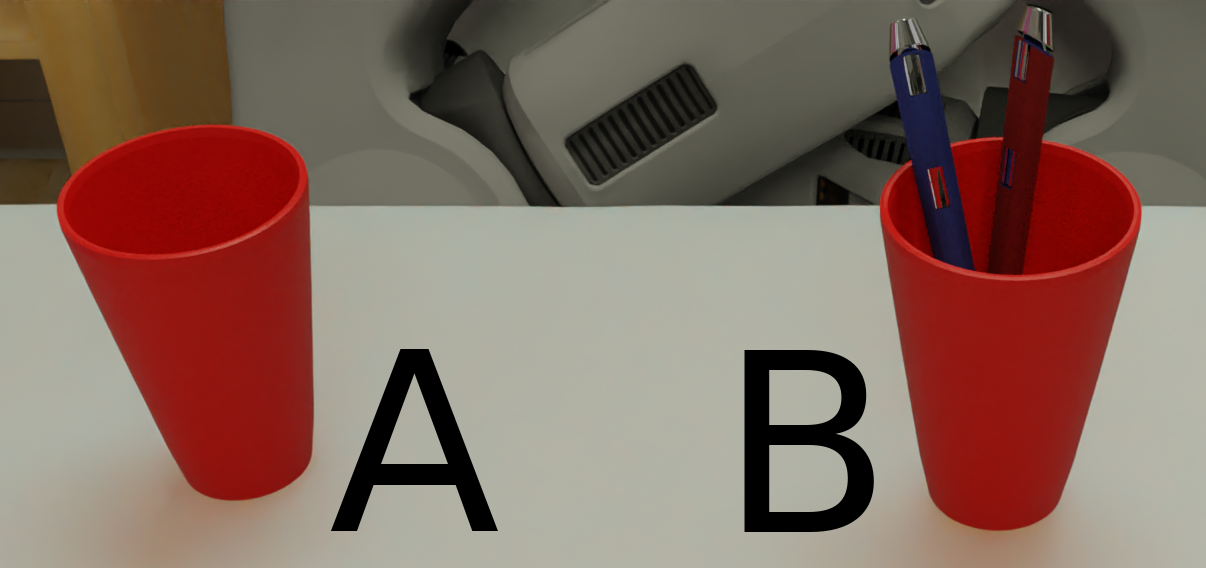
\includegraphics[scale=0.15]{figures/chapter4/complet_validity.png}
\caption{\label{fig:chap4_complet} A situation where referring to the cup B through realtions to the pens can be done either by leaving the ambiguity on the pen (minimally valid RE) or also disambiguating the color of the pen (completely valid RE). }
\end{figure}

With regard to the presentend constraints, a solution to a REG problem is define as follow:

\begin{definition}[Referring Expression Generation solution]
A solution to the REG problem is thus $\solution = \langle E, \var_t \rangle$, with $E$ a valid referring expression in the form of a set of under-specified relations representing the \sparql{} query and $\var_t$ the variable designating the target entity $\goalindiv$.
\end{definition}


Finally, considering the fact that some relations are easier to understand than others, we can define the relations cost function\footnote{The cost function is here seen as a black-box which can be a static map, the result of a learning process or other.} $\costfunc : \relationset \rightarrow \mathbb{R}^+$. Thanks to it, we can define an optimal solution to a REG problem.

\begin{definition}[Optimal Referring Expression Generation solution]
The optimal solution $\solution^* = \langle E^*, \var_t \rangle$ is thus the solution minimizing $\sum_{\relation \in E^*} \costfunc(\relation)$ over the set of all the possible solutions for a REG problem.
\end{definition}



\section{Uniform Cost Search REG}

In the previous section, we have defined a Referring Expression Generation problem as well as its solution. In this section, we first formalise this problem as a search problem and we then present an algorithm abe to solve it in a smart way.

\subsection{Formalisation as a search problem}

In the REG problem, we can consider a \textbf{candidate Referring Expression} as a \textbf{state} $\state$ of a search algorithm. A candidate RE is a RE under construction that does not respect all the constraints to make a valid RE. It is a set $\mathcal{T} \subseteq \relationset \cup C$ of relation $\relation$ representing relations present in the referenced knowledge base $\kbs$. The \textbf{initial state} is specified by the context of the problem that is a set of relations that we assume to be already known by the hearer.
%\footnote{If you do not understand why we use a set of relations while we said that a RE in s set of under-specified relations in the form of a $\sparql{}$ query, just remember that we can easily go from one to the other.}

To find all the entities referred by a candidate RE, we transform it into a \sparql{} query by replacing the anonymous entities with variables. We then submit it to the ontology to know which entities can be bound to each variable of the query. Depending on whether the result of the query gives the correct matches between variables and entities or not, we can know if a state is a \textbf{target state} or not. A state is a target state id the variables to entities matching make the RE valid (minimally or completely regarding our needs).

An \textbf{action} $\action$ in the REG problem consists in the insertion of a new triplet $(\subject, \property, \object)$ to the set $\mathcal{T}$ of a state $\state$. Performing an action on state results in the creation of a new state $\state'$. The inserted triplet can represent an entity type (coming from $\inheritset$) or a relation between entities (coming from $\relationset$). When it represents an entity type, we call the action a \textbf{typing action} with $\property \equiv isA$. When it is a relation coming from the relation set $\relationset$, we want it to reduce the existing ambiguity in a given state. we thus aim the relation to differs between ambiguous entities in $\state$. In this case, we call the action a \textbf{difference action}. To consider the open-world assumption, we can refine this difference in two categories:

\begin{definition}[Hard difference]
An hard difference exists when two entities own the same property towards a different entity: $(\indiv_i, \property, \object_i) \in \relationset \land (\indiv_j, \property, \object_j) \in \relationset | \object_i \neq \object_j$. We note this difference between two entities ($\indiv_i, \harddiff, \indiv_j$).
\end{definition}

\begin{definition}[Soft difference]
A soft difference exists when an entity owns a property that is not owned by another ambiguous entity: $(\indiv_1, \property, \object_i) \in \relationset \land (\indiv_j, \property, \cdot) \notin \relationset$. We note this difference between two entities ($\indiv_i, \softdiff, \indiv_j$).
\end{definition}

Considering the Figure.\ref{fig:chap4_complet} with the two pens, it exists a hard difference between the two pens regarding their color as one is blue and the other is red. The two pens own a relation with the same property \textit{hasColor} but on different entities, red and blue. A soft difference exists between the two cups as cup B has something inside and not cup A.

To represent the fact that some referring expressions are easier to understand than others depending on the property they use, we define a \textbf{cost} for each state. It is the sum of the cost of the properties used in the relations of the candidate RE. The cost can thus be regardless assigned to the property of the relation or the relation itself and the cost of an action is the cost of the relation it inserts. If we assume a state $\state$ with a cost $\cost$, performing an action $\action_j$ corresponds to the fact of adding a relation $\relation_j$ and create a new state $\state'$. The cost of this new state can be calculated either from the cost of the previous state $\cost' = \cost + \costfunc(\relation_j)$ or independently $\cost' = \sum_{\relation \in \mathcal{T}} \costfunc(\relation)$. In addition, as the hard differences respect the open-world assumption ut the soft differences do not, we propose to encourage the use of hard difference when possible by adding an extra cost to relations coming from soft differences.

To manage the REG problem as a search problem, we finally define a search \textbf{node} $\node$ that is, at least, composed of a candidate RE (thus a state) $\state$ and a cost $\cost$.

\subsection{Algorithm choice}

We consider the REG problem to be a graph search problem when we perform it on an ontology. If we had considered a state $\state'$ as being composed only of the relation provided by the action $\action$ from state $\state$, a tree search should have been used because state $\state'$ would depend on state $\state$. Considering a state as being a set $\mathcal{T}$ of relations $\relation$, the states become independent of each other and can be compared as $\mathcal{T}_x = \mathcal{T}_y$ iff $\forall{z},(z\in \mathcal{T}_x \Leftrightarrow z\in \mathcal{T}_y)$.

From any state, we can compute the number of pending ambiguous entities. We could think that this knowledge beyond the problem definition could be used to drive the searc. However, when we say that it still has X ambiguous individuals this means that the algorithm will have to perform at most X actions to reach a target state. This means that the heuristic function would overestimate the cost to reach the goal. In this sense, a such heuristic is not admissible and informed search is not applicable.

Although we could define the reverse actions that is to remove remations from a state, we do not know any solution of the problem and therefore we cannot do a backward search from it.

Taking a look to breath-first search, it is optimal when all steps costs are equal because it always expands the shallowest unexpanded node. However, in the REG problem, actions do not have the same cost as explained previously to represent the preference over features. In this case, the breadth-first search is not optimal and is therefore not suited to our problem.

At the difference of the breadth-first search, the \textbf{uniform-cost search} (UCS) expands the node with the lowest cost. That allows us to take advantage of the preference over features to find efficietly the optimal solution. Indeed, is \textbf{optimal} and \textbf{complete} with positive action costs and a finite number of entities and properties in $\kb$.

\subsection{Algorithm presentation}

Our REG algorithm performs a graph search in the space of states, using the Uniform-Cost Seach algorithm presented in Algorithm~\ref{alg:chap4_ucs}.
From an initial state, built from the context of the query, the algorithm generates a set of actions that add relations to the current state and create new states to explore. Just like Dijkstra's algorithm, it expands the states in increasing cost order until a solution is discovered or the search space is exhausted. We can however note a slight difference with the original algorithm. Because in our case two candidates RE said to be equivalent (i.e. owning the same relations regardless of their order) always have the same cost, we do not need to replace in the frontier a node with an equivalent state but having a higher cost than the newly created child node.

\newcommand{\tovariable}{\textsc{ToVariable}}
\newcommand{\toquery}{\textsc{ToQuery}}
\newcommand{\sparqlresult}{\textsc{SparqlResult}}
\newcommand{\createchild}{\textsc{CreateChild}}
\newcommand{\actions}{\textsc{Actions}}
\newcommand{\goaltest}{\textsc{GoalTest}}
\newcommand{\typingactions}{\textsc{TypingActions}}
\newcommand{\differenceactions}{\textsc{DifferencegActions}}

\begin{algorithm}[!htbp]
\caption{Uniform-Cost Search algorithm for Referring Expression Generation}
\label{alg:chap4_ucs}
\begin{algorithmic}
\Function{UCS\_REG}{$problem$} 
    \State $node\leftarrow$ a node with RE = \textsc{create-initial-re}(\textit{problem}.context), \textit{cost} = 0
    \State $frontier\leftarrow$ a priority queue of nodes ordered by their \textit{cost}
    \State $frontier\leftarrow$ \textsc{INSERT}($node$, $frontier$)
    \State $explored\leftarrow$ an empty set
    \\
    \Loop
        \If{\textsc{empty}($frontier$)} 
        	\State \Return failure
        \EndIf
        \\
        \State $node\leftarrow$ \textsc{pop}($frontier$)
        \If{\goaltest($problem$, \toquery($node$))} 
        	\State \Return \textsc{SOLUTION}($node$)
        \EndIf
        \\
        \State add $node.RE$ to $explored$
        \ForAll{$action$ in \actions($node$)}
            \State $child \leftarrow \createchild(node, action)$
            \If{$child.RE$ is not in $explored$ or $frontier$}
            	\State $frontier\leftarrow$ \textsc{INSERT}($child$, $frontier$)
            \EndIf
        \EndFor
    \EndLoop
\EndFunction
\end{algorithmic}
\end{algorithm}

We will now detail the functions specific to the UCS applied to the REG problem.

\textbf{\tovariable: }
We globally define a symbol table $\symboltable$ to keep track of the variables assigned to the anonymous entities. When a new anonymous entity is found, it is inserted in this symbol table with a unique variable identifier. We note $\symboltable^{-1}$ the inverse table, allowing us to retrieve the entity represented by an existing variable.

\textbf{\toquery: }
It performs the translation of a set of triplets into a \sparql{} query. To do so, anonymous entities have to be replaced by their corresponding variable. For each entity involved in the triplets to convert, they are given a string representation with the function $v(\indiv): \indivset \mapsto str$: 
\[ 
    v(\indiv) = 
    \begin{cases}
        str(\indiv),& \text{if } \alabel(\indiv) \neq \emptyset\\
        \symboltable(\indiv),& \text{otherwise}
    \end{cases} 
\]

\textbf{\sparqlresult: }
It takes a \sparql{} query as input and returns a match table $\matchtable$ in the way that $\matchtable(\var)$ is the set of entities matching the variable $\var$ in the given query. While usually the matching entities of a given variable depend on the matching entities of another one\footnote{See the example b of table~\ref{tab:REs} for an illustration of this link.}, we do not need to keep this link in our application.

\textbf{\goaltest: }
The test first fails if not all the anonymous entities involved in the tested candidate RE are typed. If this first test succeeds, the function succeeds, for a minimally valid solution, if the target entity $\goalindiv$ is the only solution to the variable $v(\goalindiv)$ in $\matchtable$. For a completely valid solution, the test succeeds if the previous test succeeds and if all the others variables of $\matchtable$ have exactly one solution.

\textbf{\createchild: } 
Creating a child node from a parent node and an action is easy to see. The \createchild function is specified in the pseudo-code of Algorithm \ref{alg:child}. 

\begin{algorithm}[H]
\caption{\label{alg:child} Child node function pseudocode}
\begin{algorithmic}
\Function{\createchild}{$action$, $parent$} 
    \State \Return a node with
    \State RE = $parent$.RE $\cup$ $action$
    \State cost = $parent$.cost + $\costfunc(action)$
\EndFunction
\end{algorithmic}
\end{algorithm}

\textbf{\actions: }
For each explored state, we consider two kinds of possible actions that we can perform on it. First, the \typingactions{} aims at proposing the addition of inheritance relations for all the anonymous entities for which no inheritance relation exists in $\mathcal{T}$. Second, the \differenceactions{}, divided into \textbf{hard difference actions} and \textbf{soft differences actions}, consists in the addition of relations that differ between the ambiguous entity for each variable in $\matchtable$.

In the \typingactions{} function (Alg.~\ref{alg:typing_action}), the function \textsc{UsableClasses} returns the most specific \textit{labeled} classes of an entity $\indiv$. In other words, it returns the set of classes $\class \in \classset$ such that $(\indiv,\class) \in C$, $\tlabel(\class) \neq \emptyset$, and
$\not\exists \class'\ s.t.\ (\class', \class) \in H \wedge \tlabel(\class') \neq \emptyset$.

\begin{algorithm}[htb!]
\caption{\label{alg:typing_action} Typing actions pseudocode}
\begin{algorithmic}

    \Function{\typingactions}{$state$} 
        
        \ForAll{$(\subject, \property, \object)$ \textbf{in} $state$}
            \If {$\alabel(\subject) = \emptyset\ \wedge \not\exists \class \text{~s.t.~} (\subject, $"isA"$,\class) \in \textit{state}$}
                \State \Return $\{\ (\subject,\text{"isA"},t)\ |\ t \in \textsc{UsableClasses}(\subject)\  \}$
            \ElsIf {$\alabel(\object) = \emptyset\ \wedge \not\exists \class \text{~s.t.~} (\object, $"isA"$,\class) \in \textit{state}$}
                \State \Return $\{\ (\object,\text{"isA"},t)\ |\ t \in \textsc{UsableClasses}(\object)\  \}$
            \EndIf
        \EndFor
        \Return OK \Comment{every anonymous entity is typed}
    \EndFunction
\end{algorithmic}
\end{algorithm}

The choice to select the most specific class differs from the one of \cite{dale_1995_computational} that prefers the least specific types also called the basic-level classes. However, using a knowledge base not specific to the REG task, it would always return the classes \textit{Object} or \textit{Thing}. This could lead to confusion for the hearer and would not help to reduce the ambiguity with other entities. Selecting the most specific thus reduce the branching factor of the algorithm as soon as possible and not impacts the completeness. Moreover, working on the estimated knowledge base of the RE hearer, we can assume that the used labels and thus concepts are known to him.

The \typingactions{} is always performed before the \differenceactions{} and this second is even not called if the first has found possible actions. We thus ensure that we do not have more than one untyped anonymous entity at the time. This particularity explains why the \typingactions{} stops at the first untyped anonymous entity. Besides, it reduces once again the branching factor. Because of the parlance need constraint, we knew that any untyped anonymous entity has to be typed to find a valid solution. It is thus useless to try to add other relation while such an entity still exists in a candidate RE. Even if, for any reason, we found ourselves in a case with multiple untyped anonymous entities at the time, each of them will be typed after the other\footnote{Typing them at once would reduce the execution time but would necessitate actions to be the insertion of a set of relations which add complexity to the algorithm for cases that should not append.}.

\begin{algorithm}[htb!]
\caption{\label{alg:diffeaction} Hard difference actions pseudocode}
\begin{algorithmic}[1]
\Function{\textsc{HardDifferenceActions}}{$state$} 
    \State $actions\leftarrow$ an empty set of actions
    \State $matches\leftarrow$ \sparqlresult(\toquery($state$))

    \ForAll{$(\var, \indiv)$ \textbf{in} matches}
        \If{$\indiv \neq \symboltable^{-1}(\var)$}
            \ForAll{$r = (\symboltable^{-1}(\var), p, o)$ \textbf{in} $\symboltable^{-1}(\var) \harddiff \indiv$} 
                \State $r_{inv}$ = $(o, Inv(p), \symboltable^{-1}(\var))$
                \If{$r \not\in state \wedge r_{inv} \not\in  state \wedge p\in U$}
                    \State $\textit{actions} \gets \textit{actions} \cup \{r\}$
                \EndIf
            \EndFor
        \EndIf
    \EndFor
    \Return $actions$
\EndFunction
\end{algorithmic}
\end{algorithm}

The \differenceactions{} function call consecutively the hard then soft differences actions functions and merge their results. The pseudo-code of the hard difference actions function is provided in Algorithm~\ref{alg:diffeaction}. The $\harddiff$ at line 6 (resp. $\softdiff$) operator returns all the relations that are hard differences (resp. soft) between two entities. In both cases, an action can be added only once and must not be present in the current state to avoid redundancy. Moreover, an action can not be added if the inverse relation to the one added is already present in the current state or proposed actions. We use the $\invset$ set defined in the knowledge base to check it. It once again avoids any redundancy. Taking the example of Figure~\ref{fig:chap4_kb}, the relation $(C\_1, isOn, T\_1)$ would be redundant if the relation $(T\_1, isUnder, C\_1)$ has been already used in the current candidate RE.

\subsection{Replanning and explaining failures}

When the hearer does not understand the referring expression, we could either repeat exactly the same sentence or be smarter and add more information than needed to help him. To do so, slight modifications have to be made to the current algorithm. In the case of replanning, the frontier and the explored set do not have to be re-initialized and in case of success, the current node has to be inserted in the explored set and the next possible actions to be found before exiting. These simple modifications are sufficient to refine a not understood RE.

When no referring expression can be found, it could be interesting to give more information about the failure to the upper process. In the case of the REG problem, it could be to give the entities still in ambiguity. With such information, an upper deliberative process could in this way act on these entities to remove the ambiguity. To do so, we just have at each step of the algorithm, to keep a track of the node having the minimum of ambiguous entities. This information is present in the matching table $\matchtable$ for each node.

\section{Results}

In this section, we present the solution found by our algorithm on the example presented in section~\ref{sec:chap4_kb}. We then challenge our algorithm on a large scale ontology representing a three-room apartment to analyse it in terms of time execution, solution length and composition. Finally, we provide comparisons with two state-of-the-art methods on their own domains.

\subsection{Solution analysis: The pen in the cup}

To familiarize with the form of the solutions and better understand how the algorithm constructs them, we first solve the example of Figure~\ref{fig:chap4_kb}. The target entity $\goalindiv$ is P\_2. The corresponding variable $\var_t$ in the \sparql{} query is denoted $?0$. We assume the general knowledge to be the Tbox of Figure~\ref{fig:chap4_kb_Tbox} and the perceived relations to be the Abox of Figure~\ref{fig:chap4_kb_Abox}.

The context of the problem is that we are speaking about objects being above the table T\_1: $Ctx = (\{(?0,\ isAbove,\ T\_1)\}, \emptyset)$. The usable properties are $\usablepropset = \{visualProp,\ geometricProp\}$. Because of the properties inclusions, the properties \textit{isIn}, \textit{hasIn}, or \textit{hasColor} are usable. The problem is thus define by $\problem = \langle P\_2, \kbs, Ctx, \usablepropset \rangle$.

Because the classes \textit{ClinkingPen} and \textit{TurningPen} do not have labels, The lowest labeled class of P\_1, P\_2, and P\_3 is \textit{Pen}. A recall of the situation and the available knowledge base on which the context and the usable properties have been applied is represented on the top of Figure~\ref{fig:chap4_search}.

\begin{figure}[h!]
\centering
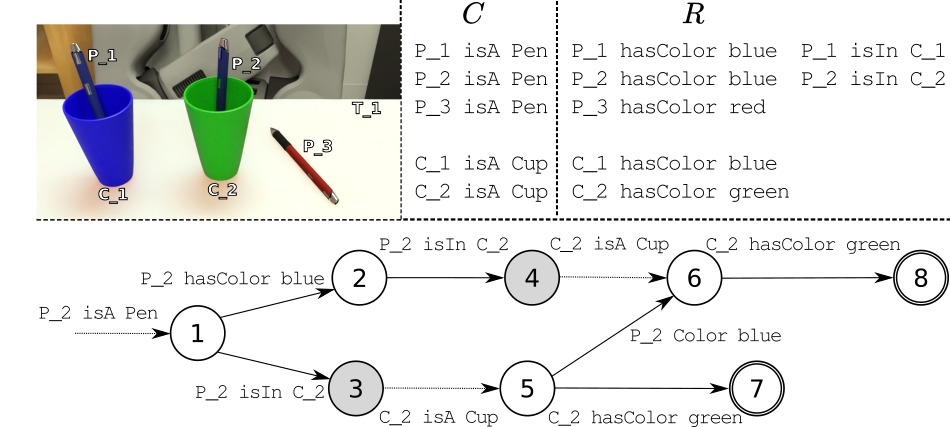
\includegraphics[scale=0.45]{figures/chapter4/search.png}
\caption{\label{fig:chap4_search} On top, a recall of the situation of Figure~\ref{fig:chap4_kb} and the entities types and relations.
At the bottom, a graphical representation of the search progress for generating a referring expression to the entity P\_2. Numbers represent the order in which the nodes are explored. Arrows are the actions performed on the nodes. Hashed arrows correspond to typing actions and greyed nodes do not respect the parlance need constraint. Double circled nodes are valid nodes. }
\end{figure}

The search process is represented at the bottom of Figure~\ref{fig:chap4_search}. It starts with node 0 in which we know that P\_2 is above the table. In this node, P\_2 is an anonymous entity and is not typed. The only possible action is thus to type it, creating node 1 with the candidate RE $\{(?0,\ isA,\ Pen)\}$. From this node, two difference actions are created and generating two new nodes. Because the action leading to node 3 introduces a new anonymous entity, it also introduces a new variable to represent it. The candidate RE related to node 3 is thus \textit{\{(?0, isA, Pen), (?0, isIn, ?1)\}}. The node with the lowest cost is explored first. In our example, all properties have a unary cost so the node to explored is selected randomly. Considering node 2 to be explored first, the entity \textit{blue} has a label so no anonymous entity has to be typed. The only possible action is that P\_2 is in the cup C\_2. Between nodes 3 and 4, node 3 has the lowest cost and is explored first. In this node, C\_2 is anonymous and not typed. The only possible action is to type C\_2. The same is done for node 4, resulting in node 6. When node 5 is explored, two difference actions are possible. However, adding the relation $(P\_2,\ hasColor,\ blue)$ to the candidate RE of node 5 results in the same state as node 6. The newly created node is thus discarded as already existing. It can also be seen as a merge of the two nodes with the same state. The second action coming from the node 5 gives the node 7 with the candidate RE \textit{\{(?0, isA, Pen), (?0, isIn, ?1), (?1, isA, Cup), (?1, hasColor, green)\}}. At this stage, the new node is just created but not evaluated. We do not know at the moment that it is a goal node. Node 6 is thus explored first and give the new node 8. Node 7 is then tested as being a goal node as the variable 0 has for only match P\_2 that is the target entity and the variable 1 can only be bound to C\_2. The algorithm does not test the node 8 has a goal node has been found.

The final solution to refer to the entity P\_2 is thus \textit{\{(?0, isA, Pen), (?0, isIn, ?1), (?1, isA, Cup), (?1, hasColor, green)\}}. It could be read as \textit{"The pen in the green cup"}. Here, we see how referring to another entity lead to interesting solutions.


\subsection{Scaling up: The three-room apartment}

\subsection{Compraritions with other state-of-the art algorithms}

\subsubsection{The longest-first}

\subsubsection{The optimized Graph Based Algorithm}

\section{Proof of concept integration on a robotic system}

\section{Integration on a robotic system}

\subsection{Verbalazing a referring expression}



\chapter*{Conclusion}
\addstarredchapter{Conclusion} %Sinon cela n'apparait pas dans la table des matières
Ce manuscrit de thèse rapporte 

%\ifdefined\included
%\else
%\bibliographystyle{acm}
%\bibliography{These-refs}
%\end{document}
%\fi


\newpage
\listoftodos[Notes]


\appendix

\chapter{Generated plans}
\label{app:plans}

\section{Compare REG with other communication means}

\begin{lstlisting}[frame=single, basicstyle=\scriptsize\ttfamily, label={lst:chap5_case3}, caption={The \acrshort{hatp} solution for the third case study of the chapter \ref{chap:5}. The robot chooses to point instead of verbalizing to designate the cubes 5 and 7. Please note the order of cube motions is not considered in this problem. The lines beginning with H represent the actions of the human and the lines beginning with HR represent actions involving the human and the robot (communication actions). In green are the \acrshort{reg} results for each communication action even if a pointing has been choose.}, captionpos=t, style=HatpPlan]
HR - TellHumanToTake(C3) // (C3, isA, Cube), (C3, hasDigit, int:1)
                         // (C3, isIn, area_red), (area_red, isA, Area),
                         // (area_red, hasColor, red)
H  - Take(C3)
HR - TellHumanToPack(C3, area_black)   // (area_black, isA, Area),
                                       // (area_black, hasColor, black)
H  - Pack(C3, area_black)


HR - TellHumanToTake(C4) // (C4, isA, Cube), (C4, hasColor, black)
                         // (C4, isIn, area_red), (area_red, isA, Area),
                         // (area_red, hasColor, red)
H  - Take(C4)
HR - TellHumanToPack(C4, area_white)   // (area_black, isA, Area),
                                       // (area_black, hasColor, white)
H  - Pack(C4, area_white)

HR - PointHumanToTake(C5) // (C5, isA, Cube), (C5, hasDigit, int:2)
                          // (C5, hasColor, black)
                          // (C5, isIn, area_black), (area_black, isA, Area),
                          // (area_black, hasColor, black)
H  - Take(C5)
HR - TellHumanToPack(C5, area_white)   // (area_black, isA, Area),
                                       // (area_black, hasColor, white)
H  - Pack(C5, area_white)

HR - TellHumanToTake(C6) // (C6, isA, Cube), (C6, hasDigit, int:2)
                         // (C6, hasColor, red)
H  - Take(C6)
HR - TellHumanToPack(C6, area_white)   // (area_black, isA, Area),
                                       // (area_black, hasColor, white)
H  - Pack(C6, area_white)

HR - PointHumanToTake(C7) // (C7, isA, Cube), (C7, hasDigit, int:2)
                          // (C7, hasColor, green)
                          // (C7, isIn, area_black), (area_black, isA, Area),
                          // (area_black, hasColor, black)
H  - Take(C7)
HR - TellHumanToPack(C7, area_white)   // (area_black, isA, Area),
                                       // (area_black, hasColor, white)
H  - Pack(C7, area_white)

HR - TellHumanToTake(C9) // (C9, isA, Cube), (C9, hasColor, black)
                         // (C9, isIn, area_black), (area_black, isA, Area),
                         // (area_black, hasColor, black)
H  - Take(C9)
HR - TellHumanToPack(C9, area_red)     // (area_red, isA, Area),
                                       // (area_red, hasColor, red)
H  - Pack(C9, area_red)

HR - PointHumanToTake(C11) // (C11, isA, Cube), (C11, hasDigit, int:1)
                           // (C11, hasColor, red)
H  - Take(C11)
HR - TellHumanToPack(C11, area_black)   // (area_black, isA, Area),
                                        // (area_black, hasColor, black)
H  - Pack(C11, area_black)
\end{lstlisting}



\bibliographystyle{StyleThese}
%\bibliographystyle{plain}
\bibliography{These-refs}

\cleardoublepage
\begin{vcenterpage}
\noindent\rule[2pt]{\textwidth}{0.5pt}
\\
\iftoggle{ThesisInEnglish}{%
{\large\textbf{Abstract:}}
}{%
{\large\textbf{Résumé :}}
}
resume
\iftoggle{ThesisInEnglish}{%
{\large\textbf{Keywords:}}
}{%
{\large\textbf{Mots clés :}}
}
mots, clefs
\\
\noindent\rule[2pt]{\textwidth}{0.5pt}
\end{vcenterpage}

\end{document}
